\batchmode
\documentclass[twoside]{book}

% Packages required by doxygen
\usepackage{fixltx2e}
\usepackage{calc}
\usepackage{doxygen}
\usepackage[export]{adjustbox} % also loads graphicx
\usepackage{graphicx}
\usepackage[utf8]{inputenc}
\usepackage{makeidx}
\usepackage{multicol}
\usepackage{multirow}
\PassOptionsToPackage{warn}{textcomp}
\usepackage{textcomp}
\usepackage[nointegrals]{wasysym}
\usepackage[table]{xcolor}

% Font selection
\usepackage[T1]{fontenc}
\usepackage[scaled=.90]{helvet}
\usepackage{courier}
\usepackage{amssymb}
\usepackage{sectsty}
\renewcommand{\familydefault}{\sfdefault}
\allsectionsfont{%
  \fontseries{bc}\selectfont%
  \color{darkgray}%
}
\renewcommand{\DoxyLabelFont}{%
  \fontseries{bc}\selectfont%
  \color{darkgray}%
}
\newcommand{\+}{\discretionary{\mbox{\scriptsize$\hookleftarrow$}}{}{}}

% Page & text layout
\usepackage{geometry}
\geometry{%
  a4paper,%
  top=2.5cm,%
  bottom=2.5cm,%
  left=2.5cm,%
  right=2.5cm%
}
\tolerance=750
\hfuzz=15pt
\hbadness=750
\setlength{\emergencystretch}{15pt}
\setlength{\parindent}{0cm}
\setlength{\parskip}{3ex plus 2ex minus 2ex}
\makeatletter
\renewcommand{\paragraph}{%
  \@startsection{paragraph}{4}{0ex}{-1.0ex}{1.0ex}{%
    \normalfont\normalsize\bfseries\SS@parafont%
  }%
}
\renewcommand{\subparagraph}{%
  \@startsection{subparagraph}{5}{0ex}{-1.0ex}{1.0ex}{%
    \normalfont\normalsize\bfseries\SS@subparafont%
  }%
}
\makeatother

% Headers & footers
\usepackage{fancyhdr}
\pagestyle{fancyplain}
\fancyhead[LE]{\fancyplain{}{\bfseries\thepage}}
\fancyhead[CE]{\fancyplain{}{}}
\fancyhead[RE]{\fancyplain{}{\bfseries\leftmark}}
\fancyhead[LO]{\fancyplain{}{\bfseries\rightmark}}
\fancyhead[CO]{\fancyplain{}{}}
\fancyhead[RO]{\fancyplain{}{\bfseries\thepage}}
\fancyfoot[LE]{\fancyplain{}{}}
\fancyfoot[CE]{\fancyplain{}{}}
\fancyfoot[RE]{\fancyplain{}{\bfseries\scriptsize Generated by Doxygen }}
\fancyfoot[LO]{\fancyplain{}{\bfseries\scriptsize Generated by Doxygen }}
\fancyfoot[CO]{\fancyplain{}{}}
\fancyfoot[RO]{\fancyplain{}{}}
\renewcommand{\footrulewidth}{0.4pt}
\renewcommand{\chaptermark}[1]{%
  \markboth{#1}{}%
}
\renewcommand{\sectionmark}[1]{%
  \markright{\thesection\ #1}%
}

% Indices & bibliography
\usepackage{natbib}
\usepackage[titles]{tocloft}
\setcounter{tocdepth}{3}
\setcounter{secnumdepth}{5}
\makeindex

% Hyperlinks (required, but should be loaded last)
\usepackage{ifpdf}
\ifpdf
  \usepackage[pdftex,pagebackref=true]{hyperref}
\else
  \usepackage[ps2pdf,pagebackref=true]{hyperref}
\fi
\hypersetup{%
  colorlinks=true,%
  linkcolor=blue,%
  citecolor=blue,%
  unicode%
}

% Custom commands
\newcommand{\clearemptydoublepage}{%
  \newpage{\pagestyle{empty}\cleardoublepage}%
}

\usepackage{caption}
\captionsetup{labelsep=space,justification=centering,font={bf},singlelinecheck=off,skip=4pt,position=top}

%===== C O N T E N T S =====

\begin{document}

% Titlepage & ToC
\hypersetup{pageanchor=false,
             bookmarksnumbered=true,
             pdfencoding=unicode
            }
\pagenumbering{alph}
\pagenumbering{arabic}
\hypersetup{pageanchor=true}

%--- Begin generated contents ---
\chapter{Inline mesh generation and adaptation based on Triangle}
\label{index}\hypertarget{index}{}\hypertarget{index_q}{}\section{A few quick questions...}\label{index_q}
Since {\ttfamily oomph-\/lib} is developed as open-\/source software, any evidence that the code is being downloaded and used is very helpful for us as it helps to justify our continued work on this project.

We would therefore be extremely grateful if you could provide the information requested in the form below. Pressing the \char`\"{}submit\char`\"{} button will get you to the actual download page.

{\bfseries Note\+:} 
\begin{DoxyItemize}
\item All information will be treated as confidential. 
\item If you provide your email address and check the appropriate box we will add you to our mailing list to inform you of upgrades and bug fixes to the code. Rest assured that the mailing list is {\bfseries very low volume} -- we have better things to do than to bombard you with email. 
\item If you still feel reluctant to provide any of the information requested, feel free to enter some dummy input. The form will check that {\bfseries some} information has been entered but entering your name as \char`\"{}\+Joe Cool\char`\"{} is perfectly acceptable -- this is to discourage people from not providing the information simply because they are too lazy to type... 
\end{DoxyItemize}



 







 

 \hypertarget{index_pdf}{}\section{P\+D\+F file}\label{index_pdf}
A \href{../latex/refman.pdf}{\tt pdf version} of this document is available. \end{document}

\chapter{Namespace Index}
\section{Namespace List}
Here is a list of all namespaces with brief descriptions\+:\begin{DoxyCompactList}
\item\contentsline{section}{\hyperlink{namespaceGlobal__Physical__Variables}{Global\+\_\+\+Physical\+\_\+\+Variables} \\*Global variables that represent physical properties }{\pageref{namespaceGlobal__Physical__Variables}}{}
\item\contentsline{section}{\hyperlink{namespaceoomph}{oomph} }{\pageref{namespaceoomph}}{}
\item\contentsline{section}{\hyperlink{namespacePhysical__Variables}{Physical\+\_\+\+Variables} \\*Namespace for the solution of 2D linear shell equation }{\pageref{namespacePhysical__Variables}}{}
\end{DoxyCompactList}

\chapter{Hierarchical Index}
\section{Class Hierarchy}
This inheritance list is sorted roughly, but not completely, alphabetically\+:\begin{DoxyCompactList}
\item Problem\begin{DoxyCompactList}
\item \contentsline{section}{Unstructured\+Solid\+Problem$<$ E\+L\+E\+M\+E\+NT $>$}{\pageref{classUnstructuredSolidProblem}}{}
\end{DoxyCompactList}
\end{DoxyCompactList}

\chapter{Class Index}
\section{Class List}
Here are the classes, structs, unions and interfaces with brief descriptions\+:\begin{DoxyCompactList}
\item\contentsline{section}{\hyperlink{classPMLProblem}{P\+M\+L\+Problem$<$ E\+L\+E\+M\+E\+N\+T $>$} }{\pageref{classPMLProblem}}{}
\item\contentsline{section}{\hyperlink{classGlobalParameters_1_1TestPMLMapping}{Global\+Parameters\+::\+Test\+P\+M\+L\+Mapping} }{\pageref{classGlobalParameters_1_1TestPMLMapping}}{}
\end{DoxyCompactList}

\chapter{File Index}
\section{File List}
Here is a list of all files with brief descriptions\+:\begin{DoxyCompactList}
\item\contentsline{section}{\hyperlink{jeffery__orbit_8cc}{jeffery\+\_\+orbit.\+cc} }{\pageref{jeffery__orbit_8cc}}{}
\item\contentsline{section}{\hyperlink{jeffery__orbit_8txt__doxygenified_8h}{jeffery\+\_\+orbit.\+txt\+\_\+doxygenified.\+h} }{\pageref{jeffery__orbit_8txt__doxygenified_8h}}{}
\item\contentsline{section}{\hyperlink{my__taylor__hood__elements_8h}{my\+\_\+taylor\+\_\+hood\+\_\+elements.\+h} }{\pageref{my__taylor__hood__elements_8h}}{}
\end{DoxyCompactList}

\chapter{Namespace Documentation}
\hypertarget{namespaceoomph}{}\section{oomph Namespace Reference}
\label{namespaceoomph}\index{oomph@{oomph}}
\subsection*{Classes}
\begin{DoxyCompactItemize}
\item 
class \hyperlink{classoomph_1_1BellShellElement}{Bell\+Shell\+Element}
\begin{DoxyCompactList}\small\item\em \hyperlink{classoomph_1_1BellShellElement}{Bell\+Shell\+Element} elements are with subparametric interpolation for the function. \end{DoxyCompactList}\item 
class \hyperlink{classoomph_1_1FaceGeometry_3_01BellShellElement_3_01DIM_00_01NNODE__1D_01_4_01_4}{Face\+Geometry$<$ Bell\+Shell\+Element$<$ D\+I\+M, N\+N\+O\+D\+E\+\_\+1\+D $>$ $>$}
\item 
class \hyperlink{classoomph_1_1MyShellEquations}{My\+Shell\+Equations}
\item 
class \hyperlink{classoomph_1_1Plate}{Plate}
\begin{DoxyCompactList}\small\item\em Elliptical tube with half axes a and b. \end{DoxyCompactList}\end{DoxyCompactItemize}

\hypertarget{namespaceTanhSolnForPoisson}{}\section{Tanh\+Soln\+For\+Poisson Namespace Reference}
\label{namespaceTanhSolnForPoisson}\index{Tanh\+Soln\+For\+Poisson@{Tanh\+Soln\+For\+Poisson}}


Namespace for exact solution for Poisson equation with sharp step.  


\subsection*{Functions}
\begin{DoxyCompactItemize}
\item 
void \hyperlink{namespaceTanhSolnForPoisson_af7896e9c18ce6438c73ae2a875e8b7de}{get\+\_\+exact\+\_\+u} (const Vector$<$ double $>$ \&x, Vector$<$ double $>$ \&u)
\begin{DoxyCompactList}\small\item\em Exact solution as a Vector. \end{DoxyCompactList}\item 
void \hyperlink{namespaceTanhSolnForPoisson_af197decab980d38d2037032780723984}{get\+\_\+exact\+\_\+u} (const Vector$<$ double $>$ \&x, double \&u)
\begin{DoxyCompactList}\small\item\em Exact solution as a scalar. \end{DoxyCompactList}\item 
void \hyperlink{namespaceTanhSolnForPoisson_ae1b9d6789ff301e3d63a4e292213036c}{get\+\_\+source} (const Vector$<$ double $>$ \&x, double \&source)
\begin{DoxyCompactList}\small\item\em Source function to make it an exact solution. \end{DoxyCompactList}\end{DoxyCompactItemize}
\subsection*{Variables}
\begin{DoxyCompactItemize}
\item 
double \hyperlink{namespaceTanhSolnForPoisson_ae676ccd186d5df119cce811596d949c1}{Alpha}
\begin{DoxyCompactList}\small\item\em Parameter for steepness of step. \end{DoxyCompactList}\item 
double \hyperlink{namespaceTanhSolnForPoisson_ae07364a1d73b28e5e250bda6c8954f01}{Beta}
\begin{DoxyCompactList}\small\item\em Parameter for angle of step. \end{DoxyCompactList}\end{DoxyCompactItemize}


\subsection{Detailed Description}
Namespace for exact solution for Poisson equation with sharp step. 

\subsection{Function Documentation}
\mbox{\Hypertarget{namespaceTanhSolnForPoisson_af7896e9c18ce6438c73ae2a875e8b7de}\label{namespaceTanhSolnForPoisson_af7896e9c18ce6438c73ae2a875e8b7de}} 
\index{Tanh\+Soln\+For\+Poisson@{Tanh\+Soln\+For\+Poisson}!get\+\_\+exact\+\_\+u@{get\+\_\+exact\+\_\+u}}
\index{get\+\_\+exact\+\_\+u@{get\+\_\+exact\+\_\+u}!Tanh\+Soln\+For\+Poisson@{Tanh\+Soln\+For\+Poisson}}
\subsubsection{\texorpdfstring{get\+\_\+exact\+\_\+u()}{get\_exact\_u()}\hspace{0.1cm}{\footnotesize\ttfamily [1/2]}}
{\footnotesize\ttfamily void Tanh\+Soln\+For\+Poisson\+::get\+\_\+exact\+\_\+u (\begin{DoxyParamCaption}\item[{const Vector$<$ double $>$ \&}]{x,  }\item[{Vector$<$ double $>$ \&}]{u }\end{DoxyParamCaption})}



Exact solution as a Vector. 



Definition at line 61 of file mesh\+\_\+from\+\_\+triangle\+\_\+poisson.\+cc.



Referenced by Poisson\+Problem$<$ E\+L\+E\+M\+E\+N\+T $>$\+::actions\+\_\+before\+\_\+newton\+\_\+solve(), and Poisson\+Problem$<$ E\+L\+E\+M\+E\+N\+T $>$\+::doc\+\_\+solution().

\mbox{\Hypertarget{namespaceTanhSolnForPoisson_af197decab980d38d2037032780723984}\label{namespaceTanhSolnForPoisson_af197decab980d38d2037032780723984}} 
\index{Tanh\+Soln\+For\+Poisson@{Tanh\+Soln\+For\+Poisson}!get\+\_\+exact\+\_\+u@{get\+\_\+exact\+\_\+u}}
\index{get\+\_\+exact\+\_\+u@{get\+\_\+exact\+\_\+u}!Tanh\+Soln\+For\+Poisson@{Tanh\+Soln\+For\+Poisson}}
\subsubsection{\texorpdfstring{get\+\_\+exact\+\_\+u()}{get\_exact\_u()}\hspace{0.1cm}{\footnotesize\ttfamily [2/2]}}
{\footnotesize\ttfamily void Tanh\+Soln\+For\+Poisson\+::get\+\_\+exact\+\_\+u (\begin{DoxyParamCaption}\item[{const Vector$<$ double $>$ \&}]{x,  }\item[{double \&}]{u }\end{DoxyParamCaption})}



Exact solution as a scalar. 



Definition at line 68 of file mesh\+\_\+from\+\_\+triangle\+\_\+poisson.\+cc.

\mbox{\Hypertarget{namespaceTanhSolnForPoisson_ae1b9d6789ff301e3d63a4e292213036c}\label{namespaceTanhSolnForPoisson_ae1b9d6789ff301e3d63a4e292213036c}} 
\index{Tanh\+Soln\+For\+Poisson@{Tanh\+Soln\+For\+Poisson}!get\+\_\+source@{get\+\_\+source}}
\index{get\+\_\+source@{get\+\_\+source}!Tanh\+Soln\+For\+Poisson@{Tanh\+Soln\+For\+Poisson}}
\subsubsection{\texorpdfstring{get\+\_\+source()}{get\_source()}}
{\footnotesize\ttfamily void Tanh\+Soln\+For\+Poisson\+::get\+\_\+source (\begin{DoxyParamCaption}\item[{const Vector$<$ double $>$ \&}]{x,  }\item[{double \&}]{source }\end{DoxyParamCaption})}



Source function to make it an exact solution. 



Definition at line 75 of file mesh\+\_\+from\+\_\+triangle\+\_\+poisson.\+cc.



Referenced by main().



\subsection{Variable Documentation}
\mbox{\Hypertarget{namespaceTanhSolnForPoisson_ae676ccd186d5df119cce811596d949c1}\label{namespaceTanhSolnForPoisson_ae676ccd186d5df119cce811596d949c1}} 
\index{Tanh\+Soln\+For\+Poisson@{Tanh\+Soln\+For\+Poisson}!Alpha@{Alpha}}
\index{Alpha@{Alpha}!Tanh\+Soln\+For\+Poisson@{Tanh\+Soln\+For\+Poisson}}
\subsubsection{\texorpdfstring{Alpha}{Alpha}}
{\footnotesize\ttfamily double Tanh\+Soln\+For\+Poisson\+::\+Alpha}



Parameter for steepness of step. 



Definition at line 54 of file mesh\+\_\+from\+\_\+triangle\+\_\+poisson.\+cc.



Referenced by Poisson\+Problem$<$ E\+L\+E\+M\+E\+N\+T $>$\+::\+Poisson\+Problem().

\mbox{\Hypertarget{namespaceTanhSolnForPoisson_ae07364a1d73b28e5e250bda6c8954f01}\label{namespaceTanhSolnForPoisson_ae07364a1d73b28e5e250bda6c8954f01}} 
\index{Tanh\+Soln\+For\+Poisson@{Tanh\+Soln\+For\+Poisson}!Beta@{Beta}}
\index{Beta@{Beta}!Tanh\+Soln\+For\+Poisson@{Tanh\+Soln\+For\+Poisson}}
\subsubsection{\texorpdfstring{Beta}{Beta}}
{\footnotesize\ttfamily double Tanh\+Soln\+For\+Poisson\+::\+Beta}



Parameter for angle of step. 



Definition at line 57 of file mesh\+\_\+from\+\_\+triangle\+\_\+poisson.\+cc.



Referenced by Poisson\+Problem$<$ E\+L\+E\+M\+E\+N\+T $>$\+::\+Poisson\+Problem().


\chapter{Class Documentation}
\hypertarget{classoomph_1_1FaceGeometry_3_01ProjectableElement_3_01ELEMENT_01_4_01_4}{}\section{oomph\+:\+:Face\+Geometry$<$ Projectable\+Element$<$ E\+L\+E\+M\+E\+NT $>$ $>$ Class Template Reference}
\label{classoomph_1_1FaceGeometry_3_01ProjectableElement_3_01ELEMENT_01_4_01_4}\index{oomph\+::\+Face\+Geometry$<$ Projectable\+Element$<$ E\+L\+E\+M\+E\+N\+T $>$ $>$@{oomph\+::\+Face\+Geometry$<$ Projectable\+Element$<$ E\+L\+E\+M\+E\+N\+T $>$ $>$}}


{\ttfamily \#include $<$projection.\+h$>$}

Inheritance diagram for oomph\+:\+:Face\+Geometry$<$ Projectable\+Element$<$ E\+L\+E\+M\+E\+NT $>$ $>$\+:\begin{figure}[H]
\begin{center}
\leavevmode
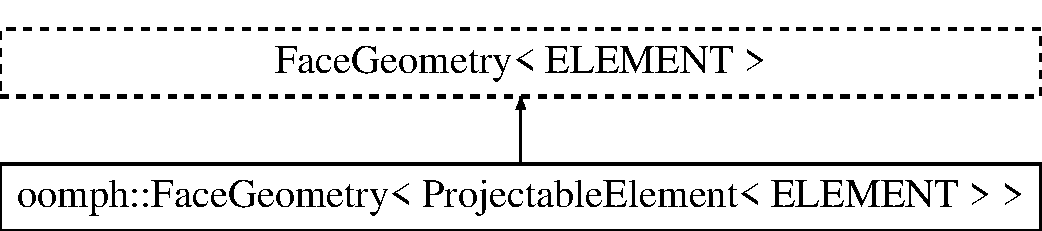
\includegraphics[height=2.000000cm]{classoomph_1_1FaceGeometry_3_01ProjectableElement_3_01ELEMENT_01_4_01_4}
\end{center}
\end{figure}
\subsection*{Public Member Functions}
\begin{DoxyCompactItemize}
\item 
\hyperlink{classoomph_1_1FaceGeometry_3_01ProjectableElement_3_01ELEMENT_01_4_01_4_a62c7dbbd61666c35f66cb028468bd110}{Face\+Geometry} ()
\end{DoxyCompactItemize}


\subsection{Detailed Description}
\subsubsection*{template$<$class E\+L\+E\+M\+E\+NT$>$\newline
class oomph\+::\+Face\+Geometry$<$ Projectable\+Element$<$ E\+L\+E\+M\+E\+N\+T $>$ $>$}

Face geometry for element is the same as that for the underlying wrapped element 

Definition at line 652 of file projection.\+h.



\subsection{Constructor \& Destructor Documentation}
\mbox{\Hypertarget{classoomph_1_1FaceGeometry_3_01ProjectableElement_3_01ELEMENT_01_4_01_4_a62c7dbbd61666c35f66cb028468bd110}\label{classoomph_1_1FaceGeometry_3_01ProjectableElement_3_01ELEMENT_01_4_01_4_a62c7dbbd61666c35f66cb028468bd110}} 
\index{oomph\+::\+Face\+Geometry$<$ Projectable\+Element$<$ E\+L\+E\+M\+E\+N\+T $>$ $>$@{oomph\+::\+Face\+Geometry$<$ Projectable\+Element$<$ E\+L\+E\+M\+E\+N\+T $>$ $>$}!Face\+Geometry@{Face\+Geometry}}
\index{Face\+Geometry@{Face\+Geometry}!oomph\+::\+Face\+Geometry$<$ Projectable\+Element$<$ E\+L\+E\+M\+E\+N\+T $>$ $>$@{oomph\+::\+Face\+Geometry$<$ Projectable\+Element$<$ E\+L\+E\+M\+E\+N\+T $>$ $>$}}
\subsubsection{\texorpdfstring{Face\+Geometry()}{FaceGeometry()}}
{\footnotesize\ttfamily template$<$class E\+L\+E\+M\+E\+NT $>$ \\
\hyperlink{classoomph_1_1FaceGeometry}{oomph\+::\+Face\+Geometry}$<$ \hyperlink{classoomph_1_1ProjectableElement}{Projectable\+Element}$<$ E\+L\+E\+M\+E\+NT $>$ $>$\+::\hyperlink{classoomph_1_1FaceGeometry}{Face\+Geometry} (\begin{DoxyParamCaption}{ }\end{DoxyParamCaption})\hspace{0.3cm}{\ttfamily [inline]}}



Definition at line 656 of file projection.\+h.



The documentation for this class was generated from the following file\+:\begin{DoxyCompactItemize}
\item 
\hyperlink{projection_8h}{projection.\+h}\end{DoxyCompactItemize}

\hypertarget{classoomph_1_1ProjectableElement}{}\section{oomph\+:\+:Projectable\+Element$<$ E\+L\+E\+M\+E\+NT $>$ Class Template Reference}
\label{classoomph_1_1ProjectableElement}\index{oomph\+::\+Projectable\+Element$<$ E\+L\+E\+M\+E\+N\+T $>$@{oomph\+::\+Projectable\+Element$<$ E\+L\+E\+M\+E\+N\+T $>$}}


{\ttfamily \#include $<$projection.\+h$>$}

Inheritance diagram for oomph\+:\+:Projectable\+Element$<$ E\+L\+E\+M\+E\+NT $>$\+:\begin{figure}[H]
\begin{center}
\leavevmode
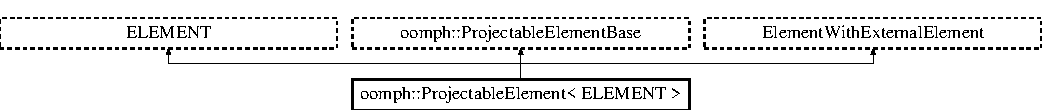
\includegraphics[height=1.475626cm]{classoomph_1_1ProjectableElement}
\end{center}
\end{figure}
\subsection*{Public Member Functions}
\begin{DoxyCompactItemize}
\item 
\hyperlink{classoomph_1_1ProjectableElement_a1892a2e757d35952be803d56078a3320}{Projectable\+Element} ()
\begin{DoxyCompactList}\small\item\em Constructor \mbox{[}this was only required explicitly from gcc 4.\+5.\+2 onwards...\mbox{]}. \end{DoxyCompactList}\item 
virtual void \hyperlink{classoomph_1_1ProjectableElement_a1ff7a9207ec5e4fc2508e75064e136de}{residual\+\_\+for\+\_\+projection} (Vector$<$ double $>$ \&residuals, Dense\+Matrix$<$ double $>$ \&jacobian, const unsigned \&flag)
\begin{DoxyCompactList}\small\item\em Residual for the projection step. Flag indicates if we want the Jacobian (1) or not (0). Virtual so it can be overloaded if necessary. \end{DoxyCompactList}\item 
double \hyperlink{classoomph_1_1ProjectableElement_aefceb50221fe76ac929d618495530adf}{zeta\+\_\+nodal} (const unsigned \&n, const unsigned \&k, const unsigned \&i) const
\begin{DoxyCompactList}\small\item\em Use Eulerian coordinates for matching in locate\+\_\+zeta when doing projection. \end{DoxyCompactList}\item 
void \hyperlink{classoomph_1_1ProjectableElement_a08968691986cf6dbe45e5c20d46e46be}{enable\+\_\+projection} ()
\begin{DoxyCompactList}\small\item\em Backup the element\textquotesingle{}s state and switch it to projection mode. \end{DoxyCompactList}\item 
void \hyperlink{classoomph_1_1ProjectableElement_afd30334bf9f7cf2e9d210b7705bd8572}{disable\+\_\+projection} ()
\begin{DoxyCompactList}\small\item\em Helper function to restore the element to the state it was in before we entered the projection mode and switch off projection mode. \end{DoxyCompactList}\item 
void \hyperlink{classoomph_1_1ProjectableElement_ada702d9b155574b33a31c3693f268887}{set\+\_\+project\+\_\+coordinates} ()
\begin{DoxyCompactList}\small\item\em Project (history values of) coordintes. \end{DoxyCompactList}\item 
void \hyperlink{classoomph_1_1ProjectableElement_a51fefa06ef9dc90ea400a0fa1711c232}{set\+\_\+project\+\_\+values} ()
\begin{DoxyCompactList}\small\item\em Project (history values of) values. \end{DoxyCompactList}\item 
void \hyperlink{classoomph_1_1ProjectableElement_ae1a46981a1ca1b4f9f1ef1783a168cf4}{set\+\_\+project\+\_\+lagrangian} ()
\begin{DoxyCompactList}\small\item\em Project (current and only values of) lagrangian coordinates. \end{DoxyCompactList}\item 
unsigned \& \hyperlink{classoomph_1_1ProjectableElement_a1d5640979b055e358f10c5a4b8cfb3b3}{projected\+\_\+field} ()
\begin{DoxyCompactList}\small\item\em Field that is currently being projected. \end{DoxyCompactList}\item 
unsigned \& \hyperlink{classoomph_1_1ProjectableElement_adabcd890a2193f3369dd8e1272f27f5b}{time\+\_\+level\+\_\+for\+\_\+projection} ()
\begin{DoxyCompactList}\small\item\em Which history value are we projecting? \end{DoxyCompactList}\item 
unsigned \& \hyperlink{classoomph_1_1ProjectableElement_a4b63733bc82062bf26be9ea0d18a7c08}{projected\+\_\+coordinate} ()
\begin{DoxyCompactList}\small\item\em When projecting the history values of the nodal coordinates, this is the coordinate we\textquotesingle{}re projecting. \end{DoxyCompactList}\item 
unsigned \& \hyperlink{classoomph_1_1ProjectableElement_a8ee3e91f6fdedeb5e6979e162437b2be}{projected\+\_\+lagrangian\+\_\+coordinate} ()
\begin{DoxyCompactList}\small\item\em When projecting the Lagrangian coordinates this is the coordinate that is being projected. \end{DoxyCompactList}\end{DoxyCompactItemize}
\subsection*{Protected Member Functions}
\begin{DoxyCompactItemize}
\item 
void \hyperlink{classoomph_1_1ProjectableElement_aeb0de899b7a5c7f498b2206ab00ef786}{fill\+\_\+in\+\_\+contribution\+\_\+to\+\_\+residuals} (Vector$<$ double $>$ \&residuals)
\begin{DoxyCompactList}\small\item\em Overloaded version of fill\+\_\+in\+\_\+contribution\+\_\+to\+\_\+residuals. \end{DoxyCompactList}\item 
void \hyperlink{classoomph_1_1ProjectableElement_a9e7e6d213f5e28d4b1e91433d4efb74c}{describe\+\_\+local\+\_\+dofs} (std\+::ostream \&out, const std\+::string \&current\+\_\+string) const
\begin{DoxyCompactList}\small\item\em Function to describe the local dofs of the element. The ostream specifies the output stream to which the description is written; the string stores the currently assembled output that is ultimately written to the output stream by Data\+::describe\+\_\+dofs(...); it is typically built up incrementally as we descend through the call hierarchy of this function when called from Problem\+::describe\+\_\+dofs(...) \end{DoxyCompactList}\item 
void \hyperlink{classoomph_1_1ProjectableElement_a5b6894eda403bd2b9d2cf1e0314d7a23}{fill\+\_\+in\+\_\+contribution\+\_\+to\+\_\+jacobian} (Vector$<$ double $>$ \&residuals, Dense\+Matrix$<$ double $>$ \&jacobian)
\begin{DoxyCompactList}\small\item\em Overloaded version of fill\+\_\+in\+\_\+contribution\+\_\+to\+\_\+jacobian. \end{DoxyCompactList}\end{DoxyCompactItemize}
\subsection*{Additional Inherited Members}


\subsection{Detailed Description}
\subsubsection*{template$<$class E\+L\+E\+M\+E\+NT$>$\newline
class oomph\+::\+Projectable\+Element$<$ E\+L\+E\+M\+E\+N\+T $>$}

Wrapper class for projectable elements. Adds \char`\"{}projectability\char`\"{} to the underlying E\+L\+E\+M\+E\+NT. 

Definition at line 179 of file projection.\+h.



\subsection{Constructor \& Destructor Documentation}
\mbox{\Hypertarget{classoomph_1_1ProjectableElement_a1892a2e757d35952be803d56078a3320}\label{classoomph_1_1ProjectableElement_a1892a2e757d35952be803d56078a3320}} 
\index{oomph\+::\+Projectable\+Element@{oomph\+::\+Projectable\+Element}!Projectable\+Element@{Projectable\+Element}}
\index{Projectable\+Element@{Projectable\+Element}!oomph\+::\+Projectable\+Element@{oomph\+::\+Projectable\+Element}}
\subsubsection{\texorpdfstring{Projectable\+Element()}{ProjectableElement()}}
{\footnotesize\ttfamily template$<$class E\+L\+E\+M\+E\+NT$>$ \\
\hyperlink{classoomph_1_1ProjectableElement}{oomph\+::\+Projectable\+Element}$<$ E\+L\+E\+M\+E\+NT $>$\+::\hyperlink{classoomph_1_1ProjectableElement}{Projectable\+Element} (\begin{DoxyParamCaption}{ }\end{DoxyParamCaption})\hspace{0.3cm}{\ttfamily [inline]}}



Constructor \mbox{[}this was only required explicitly from gcc 4.\+5.\+2 onwards...\mbox{]}. 



Definition at line 238 of file projection.\+h.



\subsection{Member Function Documentation}
\mbox{\Hypertarget{classoomph_1_1ProjectableElement_a9e7e6d213f5e28d4b1e91433d4efb74c}\label{classoomph_1_1ProjectableElement_a9e7e6d213f5e28d4b1e91433d4efb74c}} 
\index{oomph\+::\+Projectable\+Element@{oomph\+::\+Projectable\+Element}!describe\+\_\+local\+\_\+dofs@{describe\+\_\+local\+\_\+dofs}}
\index{describe\+\_\+local\+\_\+dofs@{describe\+\_\+local\+\_\+dofs}!oomph\+::\+Projectable\+Element@{oomph\+::\+Projectable\+Element}}
\subsubsection{\texorpdfstring{describe\+\_\+local\+\_\+dofs()}{describe\_local\_dofs()}}
{\footnotesize\ttfamily template$<$class E\+L\+E\+M\+E\+NT$>$ \\
void \hyperlink{classoomph_1_1ProjectableElement}{oomph\+::\+Projectable\+Element}$<$ E\+L\+E\+M\+E\+NT $>$\+::describe\+\_\+local\+\_\+dofs (\begin{DoxyParamCaption}\item[{std\+::ostream \&}]{out,  }\item[{const std\+::string \&}]{current\+\_\+string }\end{DoxyParamCaption}) const\hspace{0.3cm}{\ttfamily [inline]}, {\ttfamily [protected]}}



Function to describe the local dofs of the element. The ostream specifies the output stream to which the description is written; the string stores the currently assembled output that is ultimately written to the output stream by Data\+::describe\+\_\+dofs(...); it is typically built up incrementally as we descend through the call hierarchy of this function when called from Problem\+::describe\+\_\+dofs(...) 



Definition at line 210 of file projection.\+h.

\mbox{\Hypertarget{classoomph_1_1ProjectableElement_afd30334bf9f7cf2e9d210b7705bd8572}\label{classoomph_1_1ProjectableElement_afd30334bf9f7cf2e9d210b7705bd8572}} 
\index{oomph\+::\+Projectable\+Element@{oomph\+::\+Projectable\+Element}!disable\+\_\+projection@{disable\+\_\+projection}}
\index{disable\+\_\+projection@{disable\+\_\+projection}!oomph\+::\+Projectable\+Element@{oomph\+::\+Projectable\+Element}}
\subsubsection{\texorpdfstring{disable\+\_\+projection()}{disable\_projection()}}
{\footnotesize\ttfamily template$<$class E\+L\+E\+M\+E\+NT$>$ \\
void \hyperlink{classoomph_1_1ProjectableElement}{oomph\+::\+Projectable\+Element}$<$ E\+L\+E\+M\+E\+NT $>$\+::disable\+\_\+projection (\begin{DoxyParamCaption}{ }\end{DoxyParamCaption})\hspace{0.3cm}{\ttfamily [inline]}}



Helper function to restore the element to the state it was in before we entered the projection mode and switch off projection mode. 



Definition at line 583 of file projection.\+h.



References oomph\+::\+Projectable\+Element\+Base\+::\+Backup\+\_\+external\+\_\+geometric\+\_\+data, oomph\+::\+Projectable\+Element\+Base\+::\+Backup\+\_\+external\+\_\+interaction\+\_\+data, oomph\+::\+Projectable\+Element\+Base\+::\+Backup\+\_\+ninteraction, and oomph\+::\+Projectable\+Element\+Base\+::\+Do\+\_\+projection.

\mbox{\Hypertarget{classoomph_1_1ProjectableElement_a08968691986cf6dbe45e5c20d46e46be}\label{classoomph_1_1ProjectableElement_a08968691986cf6dbe45e5c20d46e46be}} 
\index{oomph\+::\+Projectable\+Element@{oomph\+::\+Projectable\+Element}!enable\+\_\+projection@{enable\+\_\+projection}}
\index{enable\+\_\+projection@{enable\+\_\+projection}!oomph\+::\+Projectable\+Element@{oomph\+::\+Projectable\+Element}}
\subsubsection{\texorpdfstring{enable\+\_\+projection()}{enable\_projection()}}
{\footnotesize\ttfamily template$<$class E\+L\+E\+M\+E\+NT$>$ \\
void \hyperlink{classoomph_1_1ProjectableElement}{oomph\+::\+Projectable\+Element}$<$ E\+L\+E\+M\+E\+NT $>$\+::enable\+\_\+projection (\begin{DoxyParamCaption}{ }\end{DoxyParamCaption})\hspace{0.3cm}{\ttfamily [inline]}}



Backup the element\textquotesingle{}s state and switch it to projection mode. 



Definition at line 548 of file projection.\+h.



References oomph\+::\+Projectable\+Element\+Base\+::\+Backup\+\_\+external\+\_\+geometric\+\_\+data, oomph\+::\+Projectable\+Element\+Base\+::\+Backup\+\_\+external\+\_\+interaction\+\_\+data, oomph\+::\+Projectable\+Element\+Base\+::\+Backup\+\_\+ninteraction, and oomph\+::\+Projectable\+Element\+Base\+::\+Do\+\_\+projection.

\mbox{\Hypertarget{classoomph_1_1ProjectableElement_a5b6894eda403bd2b9d2cf1e0314d7a23}\label{classoomph_1_1ProjectableElement_a5b6894eda403bd2b9d2cf1e0314d7a23}} 
\index{oomph\+::\+Projectable\+Element@{oomph\+::\+Projectable\+Element}!fill\+\_\+in\+\_\+contribution\+\_\+to\+\_\+jacobian@{fill\+\_\+in\+\_\+contribution\+\_\+to\+\_\+jacobian}}
\index{fill\+\_\+in\+\_\+contribution\+\_\+to\+\_\+jacobian@{fill\+\_\+in\+\_\+contribution\+\_\+to\+\_\+jacobian}!oomph\+::\+Projectable\+Element@{oomph\+::\+Projectable\+Element}}
\subsubsection{\texorpdfstring{fill\+\_\+in\+\_\+contribution\+\_\+to\+\_\+jacobian()}{fill\_in\_contribution\_to\_jacobian()}}
{\footnotesize\ttfamily template$<$class E\+L\+E\+M\+E\+NT$>$ \\
void \hyperlink{classoomph_1_1ProjectableElement}{oomph\+::\+Projectable\+Element}$<$ E\+L\+E\+M\+E\+NT $>$\+::fill\+\_\+in\+\_\+contribution\+\_\+to\+\_\+jacobian (\begin{DoxyParamCaption}\item[{Vector$<$ double $>$ \&}]{residuals,  }\item[{Dense\+Matrix$<$ double $>$ \&}]{jacobian }\end{DoxyParamCaption})\hspace{0.3cm}{\ttfamily [inline]}, {\ttfamily [protected]}}



Overloaded version of fill\+\_\+in\+\_\+contribution\+\_\+to\+\_\+jacobian. 



Definition at line 218 of file projection.\+h.



References oomph\+::\+Projectable\+Element\+Base\+::\+Do\+\_\+projection.

\mbox{\Hypertarget{classoomph_1_1ProjectableElement_aeb0de899b7a5c7f498b2206ab00ef786}\label{classoomph_1_1ProjectableElement_aeb0de899b7a5c7f498b2206ab00ef786}} 
\index{oomph\+::\+Projectable\+Element@{oomph\+::\+Projectable\+Element}!fill\+\_\+in\+\_\+contribution\+\_\+to\+\_\+residuals@{fill\+\_\+in\+\_\+contribution\+\_\+to\+\_\+residuals}}
\index{fill\+\_\+in\+\_\+contribution\+\_\+to\+\_\+residuals@{fill\+\_\+in\+\_\+contribution\+\_\+to\+\_\+residuals}!oomph\+::\+Projectable\+Element@{oomph\+::\+Projectable\+Element}}
\subsubsection{\texorpdfstring{fill\+\_\+in\+\_\+contribution\+\_\+to\+\_\+residuals()}{fill\_in\_contribution\_to\_residuals()}}
{\footnotesize\ttfamily template$<$class E\+L\+E\+M\+E\+NT$>$ \\
void \hyperlink{classoomph_1_1ProjectableElement}{oomph\+::\+Projectable\+Element}$<$ E\+L\+E\+M\+E\+NT $>$\+::fill\+\_\+in\+\_\+contribution\+\_\+to\+\_\+residuals (\begin{DoxyParamCaption}\item[{Vector$<$ double $>$ \&}]{residuals }\end{DoxyParamCaption})\hspace{0.3cm}{\ttfamily [inline]}, {\ttfamily [protected]}}



Overloaded version of fill\+\_\+in\+\_\+contribution\+\_\+to\+\_\+residuals. 



Definition at line 187 of file projection.\+h.



References oomph\+::\+Projectable\+Element\+Base\+::\+Do\+\_\+projection.

\mbox{\Hypertarget{classoomph_1_1ProjectableElement_a4b63733bc82062bf26be9ea0d18a7c08}\label{classoomph_1_1ProjectableElement_a4b63733bc82062bf26be9ea0d18a7c08}} 
\index{oomph\+::\+Projectable\+Element@{oomph\+::\+Projectable\+Element}!projected\+\_\+coordinate@{projected\+\_\+coordinate}}
\index{projected\+\_\+coordinate@{projected\+\_\+coordinate}!oomph\+::\+Projectable\+Element@{oomph\+::\+Projectable\+Element}}
\subsubsection{\texorpdfstring{projected\+\_\+coordinate()}{projected\_coordinate()}}
{\footnotesize\ttfamily template$<$class E\+L\+E\+M\+E\+NT$>$ \\
unsigned\& \hyperlink{classoomph_1_1ProjectableElement}{oomph\+::\+Projectable\+Element}$<$ E\+L\+E\+M\+E\+NT $>$\+::projected\+\_\+coordinate (\begin{DoxyParamCaption}{ }\end{DoxyParamCaption})\hspace{0.3cm}{\ttfamily [inline]}}



When projecting the history values of the nodal coordinates, this is the coordinate we\textquotesingle{}re projecting. 



Definition at line 632 of file projection.\+h.



References oomph\+::\+Projectable\+Element\+Base\+::\+Projected\+\_\+coordinate.

\mbox{\Hypertarget{classoomph_1_1ProjectableElement_a1d5640979b055e358f10c5a4b8cfb3b3}\label{classoomph_1_1ProjectableElement_a1d5640979b055e358f10c5a4b8cfb3b3}} 
\index{oomph\+::\+Projectable\+Element@{oomph\+::\+Projectable\+Element}!projected\+\_\+field@{projected\+\_\+field}}
\index{projected\+\_\+field@{projected\+\_\+field}!oomph\+::\+Projectable\+Element@{oomph\+::\+Projectable\+Element}}
\subsubsection{\texorpdfstring{projected\+\_\+field()}{projected\_field()}}
{\footnotesize\ttfamily template$<$class E\+L\+E\+M\+E\+NT$>$ \\
unsigned\& \hyperlink{classoomph_1_1ProjectableElement}{oomph\+::\+Projectable\+Element}$<$ E\+L\+E\+M\+E\+NT $>$\+::projected\+\_\+field (\begin{DoxyParamCaption}{ }\end{DoxyParamCaption})\hspace{0.3cm}{\ttfamily [inline]}}



Field that is currently being projected. 



Definition at line 623 of file projection.\+h.



References oomph\+::\+Projectable\+Element\+Base\+::\+Projected\+\_\+field.

\mbox{\Hypertarget{classoomph_1_1ProjectableElement_a8ee3e91f6fdedeb5e6979e162437b2be}\label{classoomph_1_1ProjectableElement_a8ee3e91f6fdedeb5e6979e162437b2be}} 
\index{oomph\+::\+Projectable\+Element@{oomph\+::\+Projectable\+Element}!projected\+\_\+lagrangian\+\_\+coordinate@{projected\+\_\+lagrangian\+\_\+coordinate}}
\index{projected\+\_\+lagrangian\+\_\+coordinate@{projected\+\_\+lagrangian\+\_\+coordinate}!oomph\+::\+Projectable\+Element@{oomph\+::\+Projectable\+Element}}
\subsubsection{\texorpdfstring{projected\+\_\+lagrangian\+\_\+coordinate()}{projected\_lagrangian\_coordinate()}}
{\footnotesize\ttfamily template$<$class E\+L\+E\+M\+E\+NT$>$ \\
unsigned\& \hyperlink{classoomph_1_1ProjectableElement}{oomph\+::\+Projectable\+Element}$<$ E\+L\+E\+M\+E\+NT $>$\+::projected\+\_\+lagrangian\+\_\+coordinate (\begin{DoxyParamCaption}{ }\end{DoxyParamCaption})\hspace{0.3cm}{\ttfamily [inline]}}



When projecting the Lagrangian coordinates this is the coordinate that is being projected. 



Definition at line 637 of file projection.\+h.



References oomph\+::\+Projectable\+Element\+Base\+::\+Projected\+\_\+lagrangian.

\mbox{\Hypertarget{classoomph_1_1ProjectableElement_a1ff7a9207ec5e4fc2508e75064e136de}\label{classoomph_1_1ProjectableElement_a1ff7a9207ec5e4fc2508e75064e136de}} 
\index{oomph\+::\+Projectable\+Element@{oomph\+::\+Projectable\+Element}!residual\+\_\+for\+\_\+projection@{residual\+\_\+for\+\_\+projection}}
\index{residual\+\_\+for\+\_\+projection@{residual\+\_\+for\+\_\+projection}!oomph\+::\+Projectable\+Element@{oomph\+::\+Projectable\+Element}}
\subsubsection{\texorpdfstring{residual\+\_\+for\+\_\+projection()}{residual\_for\_projection()}}
{\footnotesize\ttfamily template$<$class E\+L\+E\+M\+E\+NT$>$ \\
virtual void \hyperlink{classoomph_1_1ProjectableElement}{oomph\+::\+Projectable\+Element}$<$ E\+L\+E\+M\+E\+NT $>$\+::residual\+\_\+for\+\_\+projection (\begin{DoxyParamCaption}\item[{Vector$<$ double $>$ \&}]{residuals,  }\item[{Dense\+Matrix$<$ double $>$ \&}]{jacobian,  }\item[{const unsigned \&}]{flag }\end{DoxyParamCaption})\hspace{0.3cm}{\ttfamily [inline]}, {\ttfamily [virtual]}}



Residual for the projection step. Flag indicates if we want the Jacobian (1) or not (0). Virtual so it can be overloaded if necessary. 



Definition at line 243 of file projection.\+h.



References oomph\+::\+Projectable\+Element\+Base\+::\+Coordinate, oomph\+::\+Projectable\+Element\+Base\+::get\+\_\+field(), oomph\+::\+Projectable\+Element\+Base\+::jacobian\+\_\+and\+\_\+shape\+\_\+of\+\_\+field(), oomph\+::\+Projectable\+Element\+Base\+::\+Lagrangian, oomph\+::\+Projectable\+Element\+Base\+::local\+\_\+equation(), oomph\+::\+Projectable\+Element\+Base\+::nvalue\+\_\+of\+\_\+field(), oomph\+::\+Projectable\+Element\+Base\+::\+Projected\+\_\+coordinate, oomph\+::\+Projectable\+Element\+Base\+::\+Projected\+\_\+field, oomph\+::\+Projectable\+Element\+Base\+::\+Projected\+\_\+lagrangian, oomph\+::\+Projectable\+Element\+Base\+::\+Projection\+\_\+type, oomph\+::\+Projectable\+Element\+Base\+::\+Time\+\_\+level\+\_\+for\+\_\+projection, and oomph\+::\+Projectable\+Element\+Base\+::\+Value.

\mbox{\Hypertarget{classoomph_1_1ProjectableElement_ada702d9b155574b33a31c3693f268887}\label{classoomph_1_1ProjectableElement_ada702d9b155574b33a31c3693f268887}} 
\index{oomph\+::\+Projectable\+Element@{oomph\+::\+Projectable\+Element}!set\+\_\+project\+\_\+coordinates@{set\+\_\+project\+\_\+coordinates}}
\index{set\+\_\+project\+\_\+coordinates@{set\+\_\+project\+\_\+coordinates}!oomph\+::\+Projectable\+Element@{oomph\+::\+Projectable\+Element}}
\subsubsection{\texorpdfstring{set\+\_\+project\+\_\+coordinates()}{set\_project\_coordinates()}}
{\footnotesize\ttfamily template$<$class E\+L\+E\+M\+E\+NT$>$ \\
void \hyperlink{classoomph_1_1ProjectableElement}{oomph\+::\+Projectable\+Element}$<$ E\+L\+E\+M\+E\+NT $>$\+::set\+\_\+project\+\_\+coordinates (\begin{DoxyParamCaption}{ }\end{DoxyParamCaption})\hspace{0.3cm}{\ttfamily [inline]}}



Project (history values of) coordintes. 



Definition at line 613 of file projection.\+h.



References oomph\+::\+Projectable\+Element\+Base\+::\+Coordinate, and oomph\+::\+Projectable\+Element\+Base\+::\+Projection\+\_\+type.

\mbox{\Hypertarget{classoomph_1_1ProjectableElement_ae1a46981a1ca1b4f9f1ef1783a168cf4}\label{classoomph_1_1ProjectableElement_ae1a46981a1ca1b4f9f1ef1783a168cf4}} 
\index{oomph\+::\+Projectable\+Element@{oomph\+::\+Projectable\+Element}!set\+\_\+project\+\_\+lagrangian@{set\+\_\+project\+\_\+lagrangian}}
\index{set\+\_\+project\+\_\+lagrangian@{set\+\_\+project\+\_\+lagrangian}!oomph\+::\+Projectable\+Element@{oomph\+::\+Projectable\+Element}}
\subsubsection{\texorpdfstring{set\+\_\+project\+\_\+lagrangian()}{set\_project\_lagrangian()}}
{\footnotesize\ttfamily template$<$class E\+L\+E\+M\+E\+NT$>$ \\
void \hyperlink{classoomph_1_1ProjectableElement}{oomph\+::\+Projectable\+Element}$<$ E\+L\+E\+M\+E\+NT $>$\+::set\+\_\+project\+\_\+lagrangian (\begin{DoxyParamCaption}{ }\end{DoxyParamCaption})\hspace{0.3cm}{\ttfamily [inline]}}



Project (current and only values of) lagrangian coordinates. 



Definition at line 619 of file projection.\+h.



References oomph\+::\+Projectable\+Element\+Base\+::\+Lagrangian, and oomph\+::\+Projectable\+Element\+Base\+::\+Projection\+\_\+type.

\mbox{\Hypertarget{classoomph_1_1ProjectableElement_a51fefa06ef9dc90ea400a0fa1711c232}\label{classoomph_1_1ProjectableElement_a51fefa06ef9dc90ea400a0fa1711c232}} 
\index{oomph\+::\+Projectable\+Element@{oomph\+::\+Projectable\+Element}!set\+\_\+project\+\_\+values@{set\+\_\+project\+\_\+values}}
\index{set\+\_\+project\+\_\+values@{set\+\_\+project\+\_\+values}!oomph\+::\+Projectable\+Element@{oomph\+::\+Projectable\+Element}}
\subsubsection{\texorpdfstring{set\+\_\+project\+\_\+values()}{set\_project\_values()}}
{\footnotesize\ttfamily template$<$class E\+L\+E\+M\+E\+NT$>$ \\
void \hyperlink{classoomph_1_1ProjectableElement}{oomph\+::\+Projectable\+Element}$<$ E\+L\+E\+M\+E\+NT $>$\+::set\+\_\+project\+\_\+values (\begin{DoxyParamCaption}{ }\end{DoxyParamCaption})\hspace{0.3cm}{\ttfamily [inline]}}



Project (history values of) values. 



Definition at line 616 of file projection.\+h.



References oomph\+::\+Projectable\+Element\+Base\+::\+Projection\+\_\+type, and oomph\+::\+Projectable\+Element\+Base\+::\+Value.

\mbox{\Hypertarget{classoomph_1_1ProjectableElement_adabcd890a2193f3369dd8e1272f27f5b}\label{classoomph_1_1ProjectableElement_adabcd890a2193f3369dd8e1272f27f5b}} 
\index{oomph\+::\+Projectable\+Element@{oomph\+::\+Projectable\+Element}!time\+\_\+level\+\_\+for\+\_\+projection@{time\+\_\+level\+\_\+for\+\_\+projection}}
\index{time\+\_\+level\+\_\+for\+\_\+projection@{time\+\_\+level\+\_\+for\+\_\+projection}!oomph\+::\+Projectable\+Element@{oomph\+::\+Projectable\+Element}}
\subsubsection{\texorpdfstring{time\+\_\+level\+\_\+for\+\_\+projection()}{time\_level\_for\_projection()}}
{\footnotesize\ttfamily template$<$class E\+L\+E\+M\+E\+NT$>$ \\
unsigned\& \hyperlink{classoomph_1_1ProjectableElement}{oomph\+::\+Projectable\+Element}$<$ E\+L\+E\+M\+E\+NT $>$\+::time\+\_\+level\+\_\+for\+\_\+projection (\begin{DoxyParamCaption}{ }\end{DoxyParamCaption})\hspace{0.3cm}{\ttfamily [inline]}}



Which history value are we projecting? 



Definition at line 627 of file projection.\+h.



References oomph\+::\+Projectable\+Element\+Base\+::\+Time\+\_\+level\+\_\+for\+\_\+projection.

\mbox{\Hypertarget{classoomph_1_1ProjectableElement_aefceb50221fe76ac929d618495530adf}\label{classoomph_1_1ProjectableElement_aefceb50221fe76ac929d618495530adf}} 
\index{oomph\+::\+Projectable\+Element@{oomph\+::\+Projectable\+Element}!zeta\+\_\+nodal@{zeta\+\_\+nodal}}
\index{zeta\+\_\+nodal@{zeta\+\_\+nodal}!oomph\+::\+Projectable\+Element@{oomph\+::\+Projectable\+Element}}
\subsubsection{\texorpdfstring{zeta\+\_\+nodal()}{zeta\_nodal()}}
{\footnotesize\ttfamily template$<$class E\+L\+E\+M\+E\+NT$>$ \\
double \hyperlink{classoomph_1_1ProjectableElement}{oomph\+::\+Projectable\+Element}$<$ E\+L\+E\+M\+E\+NT $>$\+::zeta\+\_\+nodal (\begin{DoxyParamCaption}\item[{const unsigned \&}]{n,  }\item[{const unsigned \&}]{k,  }\item[{const unsigned \&}]{i }\end{DoxyParamCaption}) const\hspace{0.3cm}{\ttfamily [inline]}}



Use Eulerian coordinates for matching in locate\+\_\+zeta when doing projection. 



Definition at line 531 of file projection.\+h.



References oomph\+::\+Projectable\+Element\+Base\+::\+Do\+\_\+projection.



The documentation for this class was generated from the following file\+:\begin{DoxyCompactItemize}
\item 
\hyperlink{projection_8h}{projection.\+h}\end{DoxyCompactItemize}

\hypertarget{classoomph_1_1ProjectableElementBase}{}\section{oomph\+:\+:Projectable\+Element\+Base Class Reference}
\label{classoomph_1_1ProjectableElementBase}\index{oomph\+::\+Projectable\+Element\+Base@{oomph\+::\+Projectable\+Element\+Base}}


Template-\/free Base class for projectable elements.  




{\ttfamily \#include $<$projection.\+h$>$}

Inheritance diagram for oomph\+:\+:Projectable\+Element\+Base\+:\begin{figure}[H]
\begin{center}
\leavevmode
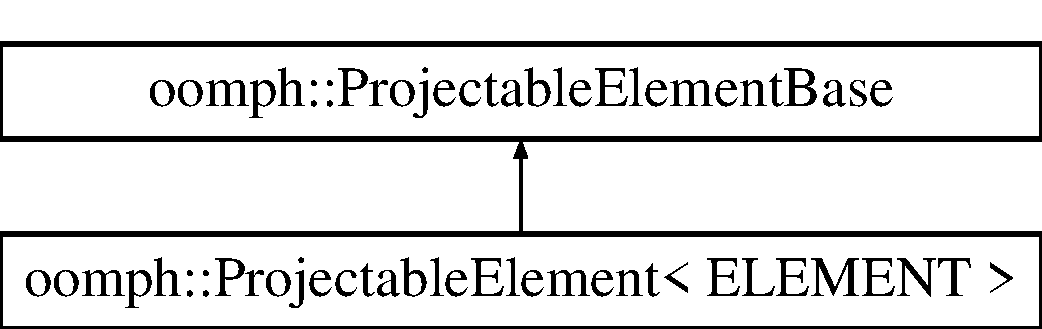
\includegraphics[height=2.000000cm]{classoomph_1_1ProjectableElementBase}
\end{center}
\end{figure}
\subsection*{Public Member Functions}
\begin{DoxyCompactItemize}
\item 
\hyperlink{classoomph_1_1ProjectableElementBase_a7ee05f9195757b46b3693786cd260ac5}{Projectable\+Element\+Base} ()
\item 
virtual \hyperlink{classoomph_1_1ProjectableElementBase_a668500db9bcaab7aa983d3c92f94e34b}{$\sim$\+Projectable\+Element\+Base} ()
\begin{DoxyCompactList}\small\item\em Virtual destructor. \end{DoxyCompactList}\item 
virtual Vector$<$ std\+::pair$<$ Data $\ast$, unsigned $>$ $>$ \hyperlink{classoomph_1_1ProjectableElementBase_a644306ebdf16f334344c2d27d72f18b7}{data\+\_\+values\+\_\+of\+\_\+field} (const unsigned \&fld)=0
\begin{DoxyCompactList}\small\item\em Pure virtual function in which the element writer must specify the values associated with field fld. The information is returned in a vector of pairs which comprise the Data object and the value within it, that correspond to field fld. E.\+g. in Taylor Hood elements the fld-\/th velocities are stored at the fld-\/th value of the nodes; the pressures (the D\+I\+M-\/th field) are the D\+I\+M-\/th values at the vertex nodes etc. \end{DoxyCompactList}\item 
virtual unsigned \hyperlink{classoomph_1_1ProjectableElementBase_a44634aa4049332a580d249c25564638c}{nfields\+\_\+for\+\_\+projection} ()=0
\begin{DoxyCompactList}\small\item\em Number of fields of the problem, so e.\+g. for 2D Navier Stokes this would be 3 (for the two velocities and one pressure) \end{DoxyCompactList}\item 
virtual unsigned \hyperlink{classoomph_1_1ProjectableElementBase_ac6790f394630b964663281f8740f43a5}{nhistory\+\_\+values\+\_\+for\+\_\+projection} (const unsigned \&fld)=0
\begin{DoxyCompactList}\small\item\em Number of history values to be stored for fld-\/th field (includes current value!) \end{DoxyCompactList}\item 
virtual unsigned \hyperlink{classoomph_1_1ProjectableElementBase_ab4ecd0cd24000a3ed675dc7198203c1f}{nhistory\+\_\+values\+\_\+for\+\_\+coordinate\+\_\+projection} ()=0
\begin{DoxyCompactList}\small\item\em Number of history values to be stored when projecting the history values of the nodal coordinates (includes current value!) \end{DoxyCompactList}\item 
virtual unsigned \hyperlink{classoomph_1_1ProjectableElementBase_a1a9a6de16f3511bca8e8be770abb9c2e}{nvalue\+\_\+of\+\_\+field} (const unsigned \&fld)=0
\begin{DoxyCompactList}\small\item\em Return number of values (pinned or not) associated with field fld within the element. This must correspond to the number of shape functions returned in jacobian\+\_\+and\+\_\+shape\+\_\+of\+\_\+field(...). \end{DoxyCompactList}\item 
virtual int \hyperlink{classoomph_1_1ProjectableElementBase_ac5c27ae929ff636dc7747fe23fd4f738}{local\+\_\+equation} (const unsigned \&fld, const unsigned \&ivalue)=0
\begin{DoxyCompactList}\small\item\em Return local equation numbers associated with value ivalue of field fld within the element. \end{DoxyCompactList}\item 
virtual double \hyperlink{classoomph_1_1ProjectableElementBase_ad45c21b58c0985d52f68ab2d79cbb488}{jacobian\+\_\+and\+\_\+shape\+\_\+of\+\_\+field} (const unsigned \&fld, const Vector$<$ double $>$ \&s, Shape \&psi)=0
\begin{DoxyCompactList}\small\item\em Return Jacobian of mapping and the shape functions associated with field fld. The number of shape functions must match the number of values specified in nvalue\+\_\+of\+\_\+field(...). For Lagrange-\/type interpolations the shape functinos are simply the \char`\"{}normal\char`\"{} nodal shape functions; if the element contains internal Data that is not associated with shape functions, simply set the corresonding shape function to 1. \end{DoxyCompactList}\item 
virtual double \hyperlink{classoomph_1_1ProjectableElementBase_ae4da5b565b6d333be2f5920f7be763cd}{get\+\_\+field} (const unsigned \&time, const unsigned \&fld, const Vector$<$ double $>$ \&s)=0
\begin{DoxyCompactList}\small\item\em Return the fld-\/th field at local coordinates s at time-\/level time (time=0\+: current value; time$>$0\+: history values) \end{DoxyCompactList}\end{DoxyCompactItemize}
\subsection*{Protected Types}
\begin{DoxyCompactItemize}
\item 
enum \hyperlink{classoomph_1_1ProjectableElementBase_aa6b28955725b5626cc4cbf0465f12a9e}{Projection\+\_\+\+Type} \{ \hyperlink{classoomph_1_1ProjectableElementBase_aa6b28955725b5626cc4cbf0465f12a9eab653154bbbdee655a7f9a666a971b614}{Coordinate}, 
\hyperlink{classoomph_1_1ProjectableElementBase_aa6b28955725b5626cc4cbf0465f12a9ea9e3decdba764ce2f6c3155676d44e38e}{Lagrangian}, 
\hyperlink{classoomph_1_1ProjectableElementBase_aa6b28955725b5626cc4cbf0465f12a9ea7923f87012a0224d8a68656e58c5474a}{Value}
 \}\begin{DoxyCompactList}\small\item\em Enumerated collection to specify which projection problem is to be solved. \end{DoxyCompactList}
\end{DoxyCompactItemize}
\subsection*{Protected Attributes}
\begin{DoxyCompactItemize}
\item 
unsigned \hyperlink{classoomph_1_1ProjectableElementBase_aa71079c0f1075ac390708063fd7d2731}{Projected\+\_\+field}
\begin{DoxyCompactList}\small\item\em Field that is currently being projected. \end{DoxyCompactList}\item 
unsigned \hyperlink{classoomph_1_1ProjectableElementBase_a4698e178e500468c0af8c37bd47d0bd3}{Time\+\_\+level\+\_\+for\+\_\+projection}
\begin{DoxyCompactList}\small\item\em Time level we are projecting (0=current values; $>$0\+: history values) \end{DoxyCompactList}\item 
unsigned \hyperlink{classoomph_1_1ProjectableElementBase_ab712be6423145fae3c23e444187db0e2}{Projected\+\_\+coordinate}
\begin{DoxyCompactList}\small\item\em When projecting the history values of the nodal coordinates, this is the coordinate we\textquotesingle{}re projecting. \end{DoxyCompactList}\item 
unsigned \hyperlink{classoomph_1_1ProjectableElementBase_a1034f9a066d1e4116f5b6acf5e5a279c}{Projected\+\_\+lagrangian}
\begin{DoxyCompactList}\small\item\em When projecting the Lagrangain coordinates indicate which coordiante is to be projected. \end{DoxyCompactList}\item 
\hyperlink{classoomph_1_1ProjectableElementBase_aa6b28955725b5626cc4cbf0465f12a9e}{Projection\+\_\+\+Type} \hyperlink{classoomph_1_1ProjectableElementBase_a1081b0f4b3633612639f92d13a187db5}{Projection\+\_\+type}
\begin{DoxyCompactList}\small\item\em Variable to indicate if we\textquotesingle{}re projecting the history values of the nodal coordinates (Coordinate) the values themselves (Value), or the Lagrangian coordinates in Solid Mechanics problems (Lagrangian) \end{DoxyCompactList}\item 
bool \hyperlink{classoomph_1_1ProjectableElementBase_a8e6db97455edb38611347e258593f592}{Do\+\_\+projection}
\begin{DoxyCompactList}\small\item\em Bool to know if we do projection or not. If false (the default) we solve the element\textquotesingle{}s \char`\"{}real\char`\"{} equations rather than the projection equations. \end{DoxyCompactList}\item 
unsigned \hyperlink{classoomph_1_1ProjectableElementBase_a638bf48f5b8dd513c18413cd3878c0d1}{Backup\+\_\+ninteraction}
\begin{DoxyCompactList}\small\item\em Store number of \char`\"{}external\char`\"{} interactions that were assigned to the element before doing the projection. \end{DoxyCompactList}\item 
bool \hyperlink{classoomph_1_1ProjectableElementBase_a907f0491ccf46f64e97365afc2fcb773}{Backup\+\_\+external\+\_\+geometric\+\_\+data}
\begin{DoxyCompactList}\small\item\em Remember if the element includes external geometric data when used in non-\/projection mode (this is temporarily disabled during the projection) \end{DoxyCompactList}\item 
bool \hyperlink{classoomph_1_1ProjectableElementBase_a0f9195c254f229b178a8844f2572c7d4}{Backup\+\_\+external\+\_\+interaction\+\_\+data}
\begin{DoxyCompactList}\small\item\em Remember if the element includes external data when used in non-\/projection mode (this is temporarily disabled during the projection) \end{DoxyCompactList}\end{DoxyCompactItemize}


\subsection{Detailed Description}
Template-\/free Base class for projectable elements. 

Definition at line 59 of file projection.\+h.



\subsection{Member Enumeration Documentation}
\mbox{\Hypertarget{classoomph_1_1ProjectableElementBase_aa6b28955725b5626cc4cbf0465f12a9e}\label{classoomph_1_1ProjectableElementBase_aa6b28955725b5626cc4cbf0465f12a9e}} 
\index{oomph\+::\+Projectable\+Element\+Base@{oomph\+::\+Projectable\+Element\+Base}!Projection\+\_\+\+Type@{Projection\+\_\+\+Type}}
\index{Projection\+\_\+\+Type@{Projection\+\_\+\+Type}!oomph\+::\+Projectable\+Element\+Base@{oomph\+::\+Projectable\+Element\+Base}}
\subsubsection{\texorpdfstring{Projection\+\_\+\+Type}{Projection\_Type}}
{\footnotesize\ttfamily enum \hyperlink{classoomph_1_1ProjectableElementBase_aa6b28955725b5626cc4cbf0465f12a9e}{oomph\+::\+Projectable\+Element\+Base\+::\+Projection\+\_\+\+Type}\hspace{0.3cm}{\ttfamily [protected]}}



Enumerated collection to specify which projection problem is to be solved. 

\begin{DoxyEnumFields}{Enumerator}
\raisebox{\heightof{T}}[0pt][0pt]{\index{Coordinate@{Coordinate}!oomph\+::\+Projectable\+Element\+Base@{oomph\+::\+Projectable\+Element\+Base}}\index{oomph\+::\+Projectable\+Element\+Base@{oomph\+::\+Projectable\+Element\+Base}!Coordinate@{Coordinate}}}\mbox{\Hypertarget{classoomph_1_1ProjectableElementBase_aa6b28955725b5626cc4cbf0465f12a9eab653154bbbdee655a7f9a666a971b614}\label{classoomph_1_1ProjectableElementBase_aa6b28955725b5626cc4cbf0465f12a9eab653154bbbdee655a7f9a666a971b614}} 
Coordinate&\\
\hline

\raisebox{\heightof{T}}[0pt][0pt]{\index{Lagrangian@{Lagrangian}!oomph\+::\+Projectable\+Element\+Base@{oomph\+::\+Projectable\+Element\+Base}}\index{oomph\+::\+Projectable\+Element\+Base@{oomph\+::\+Projectable\+Element\+Base}!Lagrangian@{Lagrangian}}}\mbox{\Hypertarget{classoomph_1_1ProjectableElementBase_aa6b28955725b5626cc4cbf0465f12a9ea9e3decdba764ce2f6c3155676d44e38e}\label{classoomph_1_1ProjectableElementBase_aa6b28955725b5626cc4cbf0465f12a9ea9e3decdba764ce2f6c3155676d44e38e}} 
Lagrangian&\\
\hline

\raisebox{\heightof{T}}[0pt][0pt]{\index{Value@{Value}!oomph\+::\+Projectable\+Element\+Base@{oomph\+::\+Projectable\+Element\+Base}}\index{oomph\+::\+Projectable\+Element\+Base@{oomph\+::\+Projectable\+Element\+Base}!Value@{Value}}}\mbox{\Hypertarget{classoomph_1_1ProjectableElementBase_aa6b28955725b5626cc4cbf0465f12a9ea7923f87012a0224d8a68656e58c5474a}\label{classoomph_1_1ProjectableElementBase_aa6b28955725b5626cc4cbf0465f12a9ea7923f87012a0224d8a68656e58c5474a}} 
Value&\\
\hline

\end{DoxyEnumFields}


Definition at line 66 of file projection.\+h.



\subsection{Constructor \& Destructor Documentation}
\mbox{\Hypertarget{classoomph_1_1ProjectableElementBase_a7ee05f9195757b46b3693786cd260ac5}\label{classoomph_1_1ProjectableElementBase_a7ee05f9195757b46b3693786cd260ac5}} 
\index{oomph\+::\+Projectable\+Element\+Base@{oomph\+::\+Projectable\+Element\+Base}!Projectable\+Element\+Base@{Projectable\+Element\+Base}}
\index{Projectable\+Element\+Base@{Projectable\+Element\+Base}!oomph\+::\+Projectable\+Element\+Base@{oomph\+::\+Projectable\+Element\+Base}}
\subsubsection{\texorpdfstring{Projectable\+Element\+Base()}{ProjectableElementBase()}}
{\footnotesize\ttfamily oomph\+::\+Projectable\+Element\+Base\+::\+Projectable\+Element\+Base (\begin{DoxyParamCaption}{ }\end{DoxyParamCaption})\hspace{0.3cm}{\ttfamily [inline]}}

Constructor\+: Initialise data so that we don\textquotesingle{}t project but solve the \char`\"{}normal\char`\"{} equations associated with the element. 

Definition at line 114 of file projection.\+h.

\mbox{\Hypertarget{classoomph_1_1ProjectableElementBase_a668500db9bcaab7aa983d3c92f94e34b}\label{classoomph_1_1ProjectableElementBase_a668500db9bcaab7aa983d3c92f94e34b}} 
\index{oomph\+::\+Projectable\+Element\+Base@{oomph\+::\+Projectable\+Element\+Base}!````~Projectable\+Element\+Base@{$\sim$\+Projectable\+Element\+Base}}
\index{````~Projectable\+Element\+Base@{$\sim$\+Projectable\+Element\+Base}!oomph\+::\+Projectable\+Element\+Base@{oomph\+::\+Projectable\+Element\+Base}}
\subsubsection{\texorpdfstring{$\sim$\+Projectable\+Element\+Base()}{~ProjectableElementBase()}}
{\footnotesize\ttfamily virtual oomph\+::\+Projectable\+Element\+Base\+::$\sim$\+Projectable\+Element\+Base (\begin{DoxyParamCaption}{ }\end{DoxyParamCaption})\hspace{0.3cm}{\ttfamily [inline]}, {\ttfamily [virtual]}}



Virtual destructor. 



Definition at line 120 of file projection.\+h.



References data\+\_\+values\+\_\+of\+\_\+field(), get\+\_\+field(), jacobian\+\_\+and\+\_\+shape\+\_\+of\+\_\+field(), local\+\_\+equation(), nfields\+\_\+for\+\_\+projection(), nhistory\+\_\+values\+\_\+for\+\_\+coordinate\+\_\+projection(), nhistory\+\_\+values\+\_\+for\+\_\+projection(), and nvalue\+\_\+of\+\_\+field().



\subsection{Member Function Documentation}
\mbox{\Hypertarget{classoomph_1_1ProjectableElementBase_a644306ebdf16f334344c2d27d72f18b7}\label{classoomph_1_1ProjectableElementBase_a644306ebdf16f334344c2d27d72f18b7}} 
\index{oomph\+::\+Projectable\+Element\+Base@{oomph\+::\+Projectable\+Element\+Base}!data\+\_\+values\+\_\+of\+\_\+field@{data\+\_\+values\+\_\+of\+\_\+field}}
\index{data\+\_\+values\+\_\+of\+\_\+field@{data\+\_\+values\+\_\+of\+\_\+field}!oomph\+::\+Projectable\+Element\+Base@{oomph\+::\+Projectable\+Element\+Base}}
\subsubsection{\texorpdfstring{data\+\_\+values\+\_\+of\+\_\+field()}{data\_values\_of\_field()}}
{\footnotesize\ttfamily virtual Vector$<$std\+::pair$<$Data$\ast$,unsigned$>$ $>$ oomph\+::\+Projectable\+Element\+Base\+::data\+\_\+values\+\_\+of\+\_\+field (\begin{DoxyParamCaption}\item[{const unsigned \&}]{fld }\end{DoxyParamCaption})\hspace{0.3cm}{\ttfamily [pure virtual]}}



Pure virtual function in which the element writer must specify the values associated with field fld. The information is returned in a vector of pairs which comprise the Data object and the value within it, that correspond to field fld. E.\+g. in Taylor Hood elements the fld-\/th velocities are stored at the fld-\/th value of the nodes; the pressures (the D\+I\+M-\/th field) are the D\+I\+M-\/th values at the vertex nodes etc. 



Referenced by $\sim$\+Projectable\+Element\+Base().

\mbox{\Hypertarget{classoomph_1_1ProjectableElementBase_ae4da5b565b6d333be2f5920f7be763cd}\label{classoomph_1_1ProjectableElementBase_ae4da5b565b6d333be2f5920f7be763cd}} 
\index{oomph\+::\+Projectable\+Element\+Base@{oomph\+::\+Projectable\+Element\+Base}!get\+\_\+field@{get\+\_\+field}}
\index{get\+\_\+field@{get\+\_\+field}!oomph\+::\+Projectable\+Element\+Base@{oomph\+::\+Projectable\+Element\+Base}}
\subsubsection{\texorpdfstring{get\+\_\+field()}{get\_field()}}
{\footnotesize\ttfamily virtual double oomph\+::\+Projectable\+Element\+Base\+::get\+\_\+field (\begin{DoxyParamCaption}\item[{const unsigned \&}]{time,  }\item[{const unsigned \&}]{fld,  }\item[{const Vector$<$ double $>$ \&}]{s }\end{DoxyParamCaption})\hspace{0.3cm}{\ttfamily [pure virtual]}}



Return the fld-\/th field at local coordinates s at time-\/level time (time=0\+: current value; time$>$0\+: history values) 



Referenced by oomph\+::\+Projectable\+Element$<$ E\+L\+E\+M\+E\+N\+T $>$\+::residual\+\_\+for\+\_\+projection(), and $\sim$\+Projectable\+Element\+Base().

\mbox{\Hypertarget{classoomph_1_1ProjectableElementBase_ad45c21b58c0985d52f68ab2d79cbb488}\label{classoomph_1_1ProjectableElementBase_ad45c21b58c0985d52f68ab2d79cbb488}} 
\index{oomph\+::\+Projectable\+Element\+Base@{oomph\+::\+Projectable\+Element\+Base}!jacobian\+\_\+and\+\_\+shape\+\_\+of\+\_\+field@{jacobian\+\_\+and\+\_\+shape\+\_\+of\+\_\+field}}
\index{jacobian\+\_\+and\+\_\+shape\+\_\+of\+\_\+field@{jacobian\+\_\+and\+\_\+shape\+\_\+of\+\_\+field}!oomph\+::\+Projectable\+Element\+Base@{oomph\+::\+Projectable\+Element\+Base}}
\subsubsection{\texorpdfstring{jacobian\+\_\+and\+\_\+shape\+\_\+of\+\_\+field()}{jacobian\_and\_shape\_of\_field()}}
{\footnotesize\ttfamily virtual double oomph\+::\+Projectable\+Element\+Base\+::jacobian\+\_\+and\+\_\+shape\+\_\+of\+\_\+field (\begin{DoxyParamCaption}\item[{const unsigned \&}]{fld,  }\item[{const Vector$<$ double $>$ \&}]{s,  }\item[{Shape \&}]{psi }\end{DoxyParamCaption})\hspace{0.3cm}{\ttfamily [pure virtual]}}



Return Jacobian of mapping and the shape functions associated with field fld. The number of shape functions must match the number of values specified in nvalue\+\_\+of\+\_\+field(...). For Lagrange-\/type interpolations the shape functinos are simply the \char`\"{}normal\char`\"{} nodal shape functions; if the element contains internal Data that is not associated with shape functions, simply set the corresonding shape function to 1. 



Referenced by oomph\+::\+Projectable\+Element$<$ E\+L\+E\+M\+E\+N\+T $>$\+::residual\+\_\+for\+\_\+projection(), and $\sim$\+Projectable\+Element\+Base().

\mbox{\Hypertarget{classoomph_1_1ProjectableElementBase_ac5c27ae929ff636dc7747fe23fd4f738}\label{classoomph_1_1ProjectableElementBase_ac5c27ae929ff636dc7747fe23fd4f738}} 
\index{oomph\+::\+Projectable\+Element\+Base@{oomph\+::\+Projectable\+Element\+Base}!local\+\_\+equation@{local\+\_\+equation}}
\index{local\+\_\+equation@{local\+\_\+equation}!oomph\+::\+Projectable\+Element\+Base@{oomph\+::\+Projectable\+Element\+Base}}
\subsubsection{\texorpdfstring{local\+\_\+equation()}{local\_equation()}}
{\footnotesize\ttfamily virtual int oomph\+::\+Projectable\+Element\+Base\+::local\+\_\+equation (\begin{DoxyParamCaption}\item[{const unsigned \&}]{fld,  }\item[{const unsigned \&}]{ivalue }\end{DoxyParamCaption})\hspace{0.3cm}{\ttfamily [pure virtual]}}



Return local equation numbers associated with value ivalue of field fld within the element. 



Referenced by oomph\+::\+Projectable\+Element$<$ E\+L\+E\+M\+E\+N\+T $>$\+::residual\+\_\+for\+\_\+projection(), and $\sim$\+Projectable\+Element\+Base().

\mbox{\Hypertarget{classoomph_1_1ProjectableElementBase_a44634aa4049332a580d249c25564638c}\label{classoomph_1_1ProjectableElementBase_a44634aa4049332a580d249c25564638c}} 
\index{oomph\+::\+Projectable\+Element\+Base@{oomph\+::\+Projectable\+Element\+Base}!nfields\+\_\+for\+\_\+projection@{nfields\+\_\+for\+\_\+projection}}
\index{nfields\+\_\+for\+\_\+projection@{nfields\+\_\+for\+\_\+projection}!oomph\+::\+Projectable\+Element\+Base@{oomph\+::\+Projectable\+Element\+Base}}
\subsubsection{\texorpdfstring{nfields\+\_\+for\+\_\+projection()}{nfields\_for\_projection()}}
{\footnotesize\ttfamily virtual unsigned oomph\+::\+Projectable\+Element\+Base\+::nfields\+\_\+for\+\_\+projection (\begin{DoxyParamCaption}{ }\end{DoxyParamCaption})\hspace{0.3cm}{\ttfamily [pure virtual]}}



Number of fields of the problem, so e.\+g. for 2D Navier Stokes this would be 3 (for the two velocities and one pressure) 



Referenced by oomph\+::\+Projection\+Problem$<$ P\+R\+O\+J\+E\+C\+T\+A\+B\+L\+E\+\_\+\+E\+L\+E\+M\+E\+N\+T $>$\+::project(), and $\sim$\+Projectable\+Element\+Base().

\mbox{\Hypertarget{classoomph_1_1ProjectableElementBase_ab4ecd0cd24000a3ed675dc7198203c1f}\label{classoomph_1_1ProjectableElementBase_ab4ecd0cd24000a3ed675dc7198203c1f}} 
\index{oomph\+::\+Projectable\+Element\+Base@{oomph\+::\+Projectable\+Element\+Base}!nhistory\+\_\+values\+\_\+for\+\_\+coordinate\+\_\+projection@{nhistory\+\_\+values\+\_\+for\+\_\+coordinate\+\_\+projection}}
\index{nhistory\+\_\+values\+\_\+for\+\_\+coordinate\+\_\+projection@{nhistory\+\_\+values\+\_\+for\+\_\+coordinate\+\_\+projection}!oomph\+::\+Projectable\+Element\+Base@{oomph\+::\+Projectable\+Element\+Base}}
\subsubsection{\texorpdfstring{nhistory\+\_\+values\+\_\+for\+\_\+coordinate\+\_\+projection()}{nhistory\_values\_for\_coordinate\_projection()}}
{\footnotesize\ttfamily virtual unsigned oomph\+::\+Projectable\+Element\+Base\+::nhistory\+\_\+values\+\_\+for\+\_\+coordinate\+\_\+projection (\begin{DoxyParamCaption}{ }\end{DoxyParamCaption})\hspace{0.3cm}{\ttfamily [pure virtual]}}



Number of history values to be stored when projecting the history values of the nodal coordinates (includes current value!) 



Referenced by oomph\+::\+Projection\+Problem$<$ P\+R\+O\+J\+E\+C\+T\+A\+B\+L\+E\+\_\+\+E\+L\+E\+M\+E\+N\+T $>$\+::project(), and $\sim$\+Projectable\+Element\+Base().

\mbox{\Hypertarget{classoomph_1_1ProjectableElementBase_ac6790f394630b964663281f8740f43a5}\label{classoomph_1_1ProjectableElementBase_ac6790f394630b964663281f8740f43a5}} 
\index{oomph\+::\+Projectable\+Element\+Base@{oomph\+::\+Projectable\+Element\+Base}!nhistory\+\_\+values\+\_\+for\+\_\+projection@{nhistory\+\_\+values\+\_\+for\+\_\+projection}}
\index{nhistory\+\_\+values\+\_\+for\+\_\+projection@{nhistory\+\_\+values\+\_\+for\+\_\+projection}!oomph\+::\+Projectable\+Element\+Base@{oomph\+::\+Projectable\+Element\+Base}}
\subsubsection{\texorpdfstring{nhistory\+\_\+values\+\_\+for\+\_\+projection()}{nhistory\_values\_for\_projection()}}
{\footnotesize\ttfamily virtual unsigned oomph\+::\+Projectable\+Element\+Base\+::nhistory\+\_\+values\+\_\+for\+\_\+projection (\begin{DoxyParamCaption}\item[{const unsigned \&}]{fld }\end{DoxyParamCaption})\hspace{0.3cm}{\ttfamily [pure virtual]}}



Number of history values to be stored for fld-\/th field (includes current value!) 



Referenced by oomph\+::\+Projection\+Problem$<$ P\+R\+O\+J\+E\+C\+T\+A\+B\+L\+E\+\_\+\+E\+L\+E\+M\+E\+N\+T $>$\+::project(), and $\sim$\+Projectable\+Element\+Base().

\mbox{\Hypertarget{classoomph_1_1ProjectableElementBase_a1a9a6de16f3511bca8e8be770abb9c2e}\label{classoomph_1_1ProjectableElementBase_a1a9a6de16f3511bca8e8be770abb9c2e}} 
\index{oomph\+::\+Projectable\+Element\+Base@{oomph\+::\+Projectable\+Element\+Base}!nvalue\+\_\+of\+\_\+field@{nvalue\+\_\+of\+\_\+field}}
\index{nvalue\+\_\+of\+\_\+field@{nvalue\+\_\+of\+\_\+field}!oomph\+::\+Projectable\+Element\+Base@{oomph\+::\+Projectable\+Element\+Base}}
\subsubsection{\texorpdfstring{nvalue\+\_\+of\+\_\+field()}{nvalue\_of\_field()}}
{\footnotesize\ttfamily virtual unsigned oomph\+::\+Projectable\+Element\+Base\+::nvalue\+\_\+of\+\_\+field (\begin{DoxyParamCaption}\item[{const unsigned \&}]{fld }\end{DoxyParamCaption})\hspace{0.3cm}{\ttfamily [pure virtual]}}



Return number of values (pinned or not) associated with field fld within the element. This must correspond to the number of shape functions returned in jacobian\+\_\+and\+\_\+shape\+\_\+of\+\_\+field(...). 



Referenced by oomph\+::\+Projectable\+Element$<$ E\+L\+E\+M\+E\+N\+T $>$\+::residual\+\_\+for\+\_\+projection(), and $\sim$\+Projectable\+Element\+Base().



\subsection{Member Data Documentation}
\mbox{\Hypertarget{classoomph_1_1ProjectableElementBase_a907f0491ccf46f64e97365afc2fcb773}\label{classoomph_1_1ProjectableElementBase_a907f0491ccf46f64e97365afc2fcb773}} 
\index{oomph\+::\+Projectable\+Element\+Base@{oomph\+::\+Projectable\+Element\+Base}!Backup\+\_\+external\+\_\+geometric\+\_\+data@{Backup\+\_\+external\+\_\+geometric\+\_\+data}}
\index{Backup\+\_\+external\+\_\+geometric\+\_\+data@{Backup\+\_\+external\+\_\+geometric\+\_\+data}!oomph\+::\+Projectable\+Element\+Base@{oomph\+::\+Projectable\+Element\+Base}}
\subsubsection{\texorpdfstring{Backup\+\_\+external\+\_\+geometric\+\_\+data}{Backup\_external\_geometric\_data}}
{\footnotesize\ttfamily bool oomph\+::\+Projectable\+Element\+Base\+::\+Backup\+\_\+external\+\_\+geometric\+\_\+data\hspace{0.3cm}{\ttfamily [protected]}}



Remember if the element includes external geometric data when used in non-\/projection mode (this is temporarily disabled during the projection) 



Definition at line 100 of file projection.\+h.



Referenced by oomph\+::\+Projectable\+Element$<$ E\+L\+E\+M\+E\+N\+T $>$\+::disable\+\_\+projection(), and oomph\+::\+Projectable\+Element$<$ E\+L\+E\+M\+E\+N\+T $>$\+::enable\+\_\+projection().

\mbox{\Hypertarget{classoomph_1_1ProjectableElementBase_a0f9195c254f229b178a8844f2572c7d4}\label{classoomph_1_1ProjectableElementBase_a0f9195c254f229b178a8844f2572c7d4}} 
\index{oomph\+::\+Projectable\+Element\+Base@{oomph\+::\+Projectable\+Element\+Base}!Backup\+\_\+external\+\_\+interaction\+\_\+data@{Backup\+\_\+external\+\_\+interaction\+\_\+data}}
\index{Backup\+\_\+external\+\_\+interaction\+\_\+data@{Backup\+\_\+external\+\_\+interaction\+\_\+data}!oomph\+::\+Projectable\+Element\+Base@{oomph\+::\+Projectable\+Element\+Base}}
\subsubsection{\texorpdfstring{Backup\+\_\+external\+\_\+interaction\+\_\+data}{Backup\_external\_interaction\_data}}
{\footnotesize\ttfamily bool oomph\+::\+Projectable\+Element\+Base\+::\+Backup\+\_\+external\+\_\+interaction\+\_\+data\hspace{0.3cm}{\ttfamily [protected]}}



Remember if the element includes external data when used in non-\/projection mode (this is temporarily disabled during the projection) 



Definition at line 106 of file projection.\+h.



Referenced by oomph\+::\+Projectable\+Element$<$ E\+L\+E\+M\+E\+N\+T $>$\+::disable\+\_\+projection(), and oomph\+::\+Projectable\+Element$<$ E\+L\+E\+M\+E\+N\+T $>$\+::enable\+\_\+projection().

\mbox{\Hypertarget{classoomph_1_1ProjectableElementBase_a638bf48f5b8dd513c18413cd3878c0d1}\label{classoomph_1_1ProjectableElementBase_a638bf48f5b8dd513c18413cd3878c0d1}} 
\index{oomph\+::\+Projectable\+Element\+Base@{oomph\+::\+Projectable\+Element\+Base}!Backup\+\_\+ninteraction@{Backup\+\_\+ninteraction}}
\index{Backup\+\_\+ninteraction@{Backup\+\_\+ninteraction}!oomph\+::\+Projectable\+Element\+Base@{oomph\+::\+Projectable\+Element\+Base}}
\subsubsection{\texorpdfstring{Backup\+\_\+ninteraction}{Backup\_ninteraction}}
{\footnotesize\ttfamily unsigned oomph\+::\+Projectable\+Element\+Base\+::\+Backup\+\_\+ninteraction\hspace{0.3cm}{\ttfamily [protected]}}



Store number of \char`\"{}external\char`\"{} interactions that were assigned to the element before doing the projection. 



Definition at line 95 of file projection.\+h.



Referenced by oomph\+::\+Projectable\+Element$<$ E\+L\+E\+M\+E\+N\+T $>$\+::disable\+\_\+projection(), and oomph\+::\+Projectable\+Element$<$ E\+L\+E\+M\+E\+N\+T $>$\+::enable\+\_\+projection().

\mbox{\Hypertarget{classoomph_1_1ProjectableElementBase_a8e6db97455edb38611347e258593f592}\label{classoomph_1_1ProjectableElementBase_a8e6db97455edb38611347e258593f592}} 
\index{oomph\+::\+Projectable\+Element\+Base@{oomph\+::\+Projectable\+Element\+Base}!Do\+\_\+projection@{Do\+\_\+projection}}
\index{Do\+\_\+projection@{Do\+\_\+projection}!oomph\+::\+Projectable\+Element\+Base@{oomph\+::\+Projectable\+Element\+Base}}
\subsubsection{\texorpdfstring{Do\+\_\+projection}{Do\_projection}}
{\footnotesize\ttfamily bool oomph\+::\+Projectable\+Element\+Base\+::\+Do\+\_\+projection\hspace{0.3cm}{\ttfamily [protected]}}



Bool to know if we do projection or not. If false (the default) we solve the element\textquotesingle{}s \char`\"{}real\char`\"{} equations rather than the projection equations. 



Definition at line 90 of file projection.\+h.



Referenced by oomph\+::\+Projectable\+Element$<$ E\+L\+E\+M\+E\+N\+T $>$\+::disable\+\_\+projection(), oomph\+::\+Projectable\+Element$<$ E\+L\+E\+M\+E\+N\+T $>$\+::enable\+\_\+projection(), oomph\+::\+Projectable\+Element$<$ E\+L\+E\+M\+E\+N\+T $>$\+::fill\+\_\+in\+\_\+contribution\+\_\+to\+\_\+jacobian(), oomph\+::\+Projectable\+Element$<$ E\+L\+E\+M\+E\+N\+T $>$\+::fill\+\_\+in\+\_\+contribution\+\_\+to\+\_\+residuals(), and oomph\+::\+Projectable\+Element$<$ E\+L\+E\+M\+E\+N\+T $>$\+::zeta\+\_\+nodal().

\mbox{\Hypertarget{classoomph_1_1ProjectableElementBase_ab712be6423145fae3c23e444187db0e2}\label{classoomph_1_1ProjectableElementBase_ab712be6423145fae3c23e444187db0e2}} 
\index{oomph\+::\+Projectable\+Element\+Base@{oomph\+::\+Projectable\+Element\+Base}!Projected\+\_\+coordinate@{Projected\+\_\+coordinate}}
\index{Projected\+\_\+coordinate@{Projected\+\_\+coordinate}!oomph\+::\+Projectable\+Element\+Base@{oomph\+::\+Projectable\+Element\+Base}}
\subsubsection{\texorpdfstring{Projected\+\_\+coordinate}{Projected\_coordinate}}
{\footnotesize\ttfamily unsigned oomph\+::\+Projectable\+Element\+Base\+::\+Projected\+\_\+coordinate\hspace{0.3cm}{\ttfamily [protected]}}



When projecting the history values of the nodal coordinates, this is the coordinate we\textquotesingle{}re projecting. 



Definition at line 76 of file projection.\+h.



Referenced by oomph\+::\+Projectable\+Element$<$ E\+L\+E\+M\+E\+N\+T $>$\+::projected\+\_\+coordinate(), and oomph\+::\+Projectable\+Element$<$ E\+L\+E\+M\+E\+N\+T $>$\+::residual\+\_\+for\+\_\+projection().

\mbox{\Hypertarget{classoomph_1_1ProjectableElementBase_aa71079c0f1075ac390708063fd7d2731}\label{classoomph_1_1ProjectableElementBase_aa71079c0f1075ac390708063fd7d2731}} 
\index{oomph\+::\+Projectable\+Element\+Base@{oomph\+::\+Projectable\+Element\+Base}!Projected\+\_\+field@{Projected\+\_\+field}}
\index{Projected\+\_\+field@{Projected\+\_\+field}!oomph\+::\+Projectable\+Element\+Base@{oomph\+::\+Projectable\+Element\+Base}}
\subsubsection{\texorpdfstring{Projected\+\_\+field}{Projected\_field}}
{\footnotesize\ttfamily unsigned oomph\+::\+Projectable\+Element\+Base\+::\+Projected\+\_\+field\hspace{0.3cm}{\ttfamily [protected]}}



Field that is currently being projected. 



Definition at line 69 of file projection.\+h.



Referenced by oomph\+::\+Projectable\+Element$<$ E\+L\+E\+M\+E\+N\+T $>$\+::projected\+\_\+field(), and oomph\+::\+Projectable\+Element$<$ E\+L\+E\+M\+E\+N\+T $>$\+::residual\+\_\+for\+\_\+projection().

\mbox{\Hypertarget{classoomph_1_1ProjectableElementBase_a1034f9a066d1e4116f5b6acf5e5a279c}\label{classoomph_1_1ProjectableElementBase_a1034f9a066d1e4116f5b6acf5e5a279c}} 
\index{oomph\+::\+Projectable\+Element\+Base@{oomph\+::\+Projectable\+Element\+Base}!Projected\+\_\+lagrangian@{Projected\+\_\+lagrangian}}
\index{Projected\+\_\+lagrangian@{Projected\+\_\+lagrangian}!oomph\+::\+Projectable\+Element\+Base@{oomph\+::\+Projectable\+Element\+Base}}
\subsubsection{\texorpdfstring{Projected\+\_\+lagrangian}{Projected\_lagrangian}}
{\footnotesize\ttfamily unsigned oomph\+::\+Projectable\+Element\+Base\+::\+Projected\+\_\+lagrangian\hspace{0.3cm}{\ttfamily [protected]}}



When projecting the Lagrangain coordinates indicate which coordiante is to be projected. 



Definition at line 80 of file projection.\+h.



Referenced by oomph\+::\+Projectable\+Element$<$ E\+L\+E\+M\+E\+N\+T $>$\+::projected\+\_\+lagrangian\+\_\+coordinate(), and oomph\+::\+Projectable\+Element$<$ E\+L\+E\+M\+E\+N\+T $>$\+::residual\+\_\+for\+\_\+projection().

\mbox{\Hypertarget{classoomph_1_1ProjectableElementBase_a1081b0f4b3633612639f92d13a187db5}\label{classoomph_1_1ProjectableElementBase_a1081b0f4b3633612639f92d13a187db5}} 
\index{oomph\+::\+Projectable\+Element\+Base@{oomph\+::\+Projectable\+Element\+Base}!Projection\+\_\+type@{Projection\+\_\+type}}
\index{Projection\+\_\+type@{Projection\+\_\+type}!oomph\+::\+Projectable\+Element\+Base@{oomph\+::\+Projectable\+Element\+Base}}
\subsubsection{\texorpdfstring{Projection\+\_\+type}{Projection\_type}}
{\footnotesize\ttfamily \hyperlink{classoomph_1_1ProjectableElementBase_aa6b28955725b5626cc4cbf0465f12a9e}{Projection\+\_\+\+Type} oomph\+::\+Projectable\+Element\+Base\+::\+Projection\+\_\+type\hspace{0.3cm}{\ttfamily [protected]}}



Variable to indicate if we\textquotesingle{}re projecting the history values of the nodal coordinates (Coordinate) the values themselves (Value), or the Lagrangian coordinates in Solid Mechanics problems (Lagrangian) 



Definition at line 85 of file projection.\+h.



Referenced by oomph\+::\+Projectable\+Element$<$ E\+L\+E\+M\+E\+N\+T $>$\+::residual\+\_\+for\+\_\+projection(), oomph\+::\+Projectable\+Element$<$ E\+L\+E\+M\+E\+N\+T $>$\+::set\+\_\+project\+\_\+coordinates(), oomph\+::\+Projectable\+Element$<$ E\+L\+E\+M\+E\+N\+T $>$\+::set\+\_\+project\+\_\+lagrangian(), and oomph\+::\+Projectable\+Element$<$ E\+L\+E\+M\+E\+N\+T $>$\+::set\+\_\+project\+\_\+values().

\mbox{\Hypertarget{classoomph_1_1ProjectableElementBase_a4698e178e500468c0af8c37bd47d0bd3}\label{classoomph_1_1ProjectableElementBase_a4698e178e500468c0af8c37bd47d0bd3}} 
\index{oomph\+::\+Projectable\+Element\+Base@{oomph\+::\+Projectable\+Element\+Base}!Time\+\_\+level\+\_\+for\+\_\+projection@{Time\+\_\+level\+\_\+for\+\_\+projection}}
\index{Time\+\_\+level\+\_\+for\+\_\+projection@{Time\+\_\+level\+\_\+for\+\_\+projection}!oomph\+::\+Projectable\+Element\+Base@{oomph\+::\+Projectable\+Element\+Base}}
\subsubsection{\texorpdfstring{Time\+\_\+level\+\_\+for\+\_\+projection}{Time\_level\_for\_projection}}
{\footnotesize\ttfamily unsigned oomph\+::\+Projectable\+Element\+Base\+::\+Time\+\_\+level\+\_\+for\+\_\+projection\hspace{0.3cm}{\ttfamily [protected]}}



Time level we are projecting (0=current values; $>$0\+: history values) 



Definition at line 72 of file projection.\+h.



Referenced by oomph\+::\+Projectable\+Element$<$ E\+L\+E\+M\+E\+N\+T $>$\+::residual\+\_\+for\+\_\+projection(), and oomph\+::\+Projectable\+Element$<$ E\+L\+E\+M\+E\+N\+T $>$\+::time\+\_\+level\+\_\+for\+\_\+projection().



The documentation for this class was generated from the following file\+:\begin{DoxyCompactItemize}
\item 
\hyperlink{projection_8h}{projection.\+h}\end{DoxyCompactItemize}

\hypertarget{classoomph_1_1ProjectionProblem}{}\section{oomph\+:\+:Projection\+Problem$<$ P\+R\+O\+J\+E\+C\+T\+A\+B\+L\+E\+\_\+\+E\+L\+E\+M\+E\+NT $>$ Class Template Reference}
\label{classoomph_1_1ProjectionProblem}\index{oomph\+::\+Projection\+Problem$<$ P\+R\+O\+J\+E\+C\+T\+A\+B\+L\+E\+\_\+\+E\+L\+E\+M\+E\+N\+T $>$@{oomph\+::\+Projection\+Problem$<$ P\+R\+O\+J\+E\+C\+T\+A\+B\+L\+E\+\_\+\+E\+L\+E\+M\+E\+N\+T $>$}}


{\ttfamily \#include $<$projection.\+h$>$}

Inheritance diagram for oomph\+:\+:Projection\+Problem$<$ P\+R\+O\+J\+E\+C\+T\+A\+B\+L\+E\+\_\+\+E\+L\+E\+M\+E\+NT $>$\+:\begin{figure}[H]
\begin{center}
\leavevmode
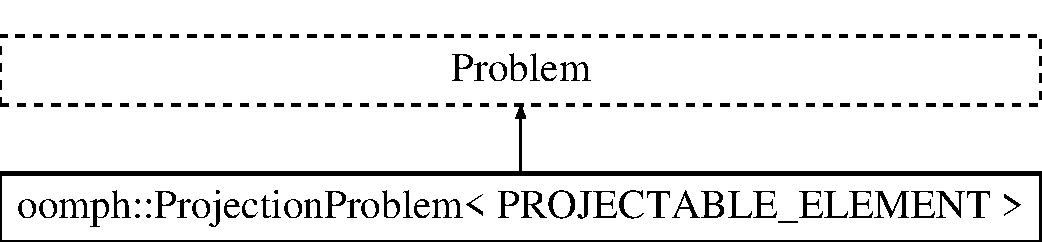
\includegraphics[height=2.000000cm]{classoomph_1_1ProjectionProblem}
\end{center}
\end{figure}
\subsection*{Public Member Functions}
\begin{DoxyCompactItemize}
\item 
void \hyperlink{classoomph_1_1ProjectionProblem_a3706c034e47193038de20f3d40443a2c}{enable\+\_\+suppress\+\_\+output\+\_\+during\+\_\+projection} ()
\begin{DoxyCompactList}\small\item\em Suppress all output during projection phases. \end{DoxyCompactList}\item 
void \hyperlink{classoomph_1_1ProjectionProblem_ab9bb57b5e9241388b4f90b37e338c454}{disable\+\_\+suppress\+\_\+output\+\_\+during\+\_\+projection} ()
\begin{DoxyCompactList}\small\item\em Undo suppression of all output during projection phases. \end{DoxyCompactList}\item 
bool \hyperlink{classoomph_1_1ProjectionProblem_a5652035eda34f398652ede076dc085ae}{use\+\_\+iterative\+\_\+solver\+\_\+for\+\_\+projection} ()
\item 
void \hyperlink{classoomph_1_1ProjectionProblem_aefda55d76d58a951ef6714cbb998e358}{enable\+\_\+use\+\_\+iterative\+\_\+solver\+\_\+for\+\_\+projection} ()
\begin{DoxyCompactList}\small\item\em Enables the use of an iterative solver for projection. \end{DoxyCompactList}\item 
void \hyperlink{classoomph_1_1ProjectionProblem_aaf4b8fcb1f5f15cd95075a7da3e76cc5}{disable\+\_\+use\+\_\+iterative\+\_\+solver\+\_\+for\+\_\+projection} ()
\begin{DoxyCompactList}\small\item\em Disbales the use of an iterative solver for projection. \end{DoxyCompactList}\item 
void \hyperlink{classoomph_1_1ProjectionProblem_ad972f78212e515a03d1018996115265a}{project} (Mesh $\ast$base\+\_\+mesh\+\_\+pt, const bool \&dont\+\_\+project\+\_\+positions=false)
\begin{DoxyCompactList}\small\item\em Project from base into the problem\textquotesingle{}s own mesh. \end{DoxyCompactList}\end{DoxyCompactItemize}
\subsection*{Private Member Functions}
\begin{DoxyCompactItemize}
\item 
\hyperlink{classoomph_1_1ProjectionProblem_a4091e944bf95ae7b3cc86ac427d93257}{Projection\+Problem} ()
\item 
\hyperlink{classoomph_1_1ProjectionProblem_a2b18253c5a5f783a329307315e9ef69c}{$\sim$\+Projection\+Problem} ()
\item 
void \hyperlink{classoomph_1_1ProjectionProblem_a5518d9926a396536ea3d24a13e0a6a71}{store\+\_\+positions} ()
\begin{DoxyCompactList}\small\item\em Helper function to store positions (the only things that have been set before doing projection. \end{DoxyCompactList}\item 
void \hyperlink{classoomph_1_1ProjectionProblem_aeb3c03ed8381f389d3d598487b6fb987}{restore\+\_\+positions} ()
\begin{DoxyCompactList}\small\item\em Helper function to restore positions (the only things that have been set before doing projection. \end{DoxyCompactList}\item 
void \hyperlink{classoomph_1_1ProjectionProblem_a9c24751d48a454956517a8541c423cf2}{pin\+\_\+all} ()
\begin{DoxyCompactList}\small\item\em Pin all the field values and position unknowns (bit inefficient) \end{DoxyCompactList}\item 
void \hyperlink{classoomph_1_1ProjectionProblem_ac0b06207d156be752a3fccfab654826e}{unpin\+\_\+all} ()
\begin{DoxyCompactList}\small\item\em Unpin all the field values and position unknowns (bit inefficient) \end{DoxyCompactList}\item 
void \hyperlink{classoomph_1_1ProjectionProblem_a50b3643c4e6942755e1ede1c0ab417ec}{unpin\+\_\+dofs\+\_\+of\+\_\+coordinate} (const unsigned \&coord)
\begin{DoxyCompactList}\small\item\em Helper function to unpin the values of coordinate coord. \end{DoxyCompactList}\item 
void \hyperlink{classoomph_1_1ProjectionProblem_ade05dce90814098ec0af15324b758730}{pin\+\_\+dofs\+\_\+of\+\_\+coordinate} (const unsigned \&coord)
\begin{DoxyCompactList}\small\item\em Helper function to unpin the values of coordinate coord. \end{DoxyCompactList}\item 
void \hyperlink{classoomph_1_1ProjectionProblem_a36847f48bff4081b5db0c038ddba1260}{unpin\+\_\+dofs\+\_\+of\+\_\+field} (const unsigned \&fld)
\begin{DoxyCompactList}\small\item\em Helper function to unpin dofs of fld-\/th field. \end{DoxyCompactList}\item 
void \hyperlink{classoomph_1_1ProjectionProblem_acff96fd0e3dda445ba806e253988c547}{pin\+\_\+dofs\+\_\+of\+\_\+field} (const unsigned \&fld)
\begin{DoxyCompactList}\small\item\em Helper function to unpin dofs of fld-\/th field. \end{DoxyCompactList}\item 
void \hyperlink{classoomph_1_1ProjectionProblem_a935983de617d4fb2feeef674af13d473}{set\+\_\+time\+\_\+level\+\_\+for\+\_\+projection} (const unsigned \&time\+\_\+level)
\begin{DoxyCompactList}\small\item\em Helper function to set time level for projection. \end{DoxyCompactList}\item 
void \hyperlink{classoomph_1_1ProjectionProblem_ad8f93fb7e51a0e427b634d4dac8e96a3}{set\+\_\+coordinate\+\_\+for\+\_\+projection} (const unsigned \&i)
\begin{DoxyCompactList}\small\item\em Set the coordinate for projection. \end{DoxyCompactList}\item 
void \hyperlink{classoomph_1_1ProjectionProblem_a944bed6fe67a6e683d3c7eb242705b6e}{set\+\_\+lagrangian\+\_\+coordinate\+\_\+for\+\_\+projection} (const unsigned \&i)
\begin{DoxyCompactList}\small\item\em Set the Lagrangian coordinate for projection. \end{DoxyCompactList}\item 
void \hyperlink{classoomph_1_1ProjectionProblem_a616f08ea08e8f1ba6be018e966f38830}{set\+\_\+current\+\_\+field\+\_\+for\+\_\+projection} (const unsigned \&fld)
\begin{DoxyCompactList}\small\item\em Set current field for projection. \end{DoxyCompactList}\end{DoxyCompactItemize}
\subsection*{Private Attributes}
\begin{DoxyCompactItemize}
\item 
Vector$<$ Dense\+Matrix$<$ double $>$ $>$ \hyperlink{classoomph_1_1ProjectionProblem_af085e8e2152466d7a98eebff07ea9271}{Solid\+\_\+backup}
\begin{DoxyCompactList}\small\item\em Backup for pin status of solid node\textquotesingle{}s position Data. \end{DoxyCompactList}\item 
bool \hyperlink{classoomph_1_1ProjectionProblem_a628ff404b240c75244eea7d38e5363dd}{Output\+\_\+during\+\_\+projection\+\_\+suppressed}
\begin{DoxyCompactList}\small\item\em Flag to suppress output during projection. \end{DoxyCompactList}\item 
bool \hyperlink{classoomph_1_1ProjectionProblem_a917be524f0312bcf05c399d7c05f95a5}{Use\+\_\+iterative\+\_\+solver\+\_\+for\+\_\+projection}
\item 
Iterative\+Linear\+Solver $\ast$ \hyperlink{classoomph_1_1ProjectionProblem_a74cb4279bf7d10be200610ca73be4d90}{Iterative\+\_\+solver\+\_\+projection\+\_\+pt}
\item 
Preconditioner $\ast$ \hyperlink{classoomph_1_1ProjectionProblem_ac351713a8fba2e5595955afaf65ab22a}{Preconditioner\+\_\+projection\+\_\+pt}
\end{DoxyCompactItemize}
\subsection*{Friends}
\begin{DoxyCompactItemize}
\item 
{\footnotesize template$<$class F\+R\+I\+E\+N\+D\+\_\+\+P\+R\+O\+J\+E\+C\+T\+A\+B\+L\+E\+\_\+\+E\+L\+E\+M\+E\+NT $>$ }\\class \hyperlink{classoomph_1_1ProjectionProblem_a13d7a9943fbdd399011c849d5839c211}{Refineable\+Triangle\+Mesh}
\item 
{\footnotesize template$<$class F\+R\+I\+E\+N\+D\+\_\+\+P\+R\+O\+J\+E\+C\+T\+A\+B\+L\+E\+\_\+\+E\+L\+E\+M\+E\+NT $>$ }\\class \hyperlink{classoomph_1_1ProjectionProblem_a999f3861375bbdf2365f6ab38447a2c4}{Refineable\+Tetgen\+Mesh}
\item 
{\footnotesize template$<$class F\+R\+I\+E\+N\+D\+\_\+\+P\+R\+O\+J\+E\+C\+T\+A\+B\+L\+E\+\_\+\+E\+L\+E\+M\+E\+NT $>$ }\\class \hyperlink{classoomph_1_1ProjectionProblem_a01ad4b9aac17e6b8e251ce52ba21bfe4}{Backup\+Mesh\+For\+Projection}
\item 
{\footnotesize template$<$class F\+R\+I\+E\+N\+D\+\_\+\+P\+R\+O\+J\+E\+C\+T\+A\+B\+L\+E\+\_\+\+E\+L\+E\+M\+E\+NT $>$ }\\class \hyperlink{classoomph_1_1ProjectionProblem_a933521be2c09eb1842625109de7a8b66}{Refineable\+Gmsh\+Tet\+Mesh}
\end{DoxyCompactItemize}


\subsection{Detailed Description}
\subsubsection*{template$<$class P\+R\+O\+J\+E\+C\+T\+A\+B\+L\+E\+\_\+\+E\+L\+E\+M\+E\+NT$>$\newline
class oomph\+::\+Projection\+Problem$<$ P\+R\+O\+J\+E\+C\+T\+A\+B\+L\+E\+\_\+\+E\+L\+E\+M\+E\+N\+T $>$}

Projection problem. This is created during the adaptation of unstructured meshes and it is assumed that no boundary conditions have been set. If they have, they will be unset during the projection and must be reset afterwards. 

Definition at line 680 of file projection.\+h.



\subsection{Constructor \& Destructor Documentation}
\mbox{\Hypertarget{classoomph_1_1ProjectionProblem_a4091e944bf95ae7b3cc86ac427d93257}\label{classoomph_1_1ProjectionProblem_a4091e944bf95ae7b3cc86ac427d93257}} 
\index{oomph\+::\+Projection\+Problem@{oomph\+::\+Projection\+Problem}!Projection\+Problem@{Projection\+Problem}}
\index{Projection\+Problem@{Projection\+Problem}!oomph\+::\+Projection\+Problem@{oomph\+::\+Projection\+Problem}}
\subsubsection{\texorpdfstring{Projection\+Problem()}{ProjectionProblem()}}
{\footnotesize\ttfamily template$<$class P\+R\+O\+J\+E\+C\+T\+A\+B\+L\+E\+\_\+\+E\+L\+E\+M\+E\+NT $>$ \\
\hyperlink{classoomph_1_1ProjectionProblem}{oomph\+::\+Projection\+Problem}$<$ P\+R\+O\+J\+E\+C\+T\+A\+B\+L\+E\+\_\+\+E\+L\+E\+M\+E\+NT $>$\+::\hyperlink{classoomph_1_1ProjectionProblem}{Projection\+Problem} (\begin{DoxyParamCaption}{ }\end{DoxyParamCaption})\hspace{0.3cm}{\ttfamily [inline]}, {\ttfamily [private]}}

Default constructor (made this private so only the friend class can call the constructor) 

Definition at line 1350 of file projection.\+h.

\mbox{\Hypertarget{classoomph_1_1ProjectionProblem_a2b18253c5a5f783a329307315e9ef69c}\label{classoomph_1_1ProjectionProblem_a2b18253c5a5f783a329307315e9ef69c}} 
\index{oomph\+::\+Projection\+Problem@{oomph\+::\+Projection\+Problem}!````~Projection\+Problem@{$\sim$\+Projection\+Problem}}
\index{````~Projection\+Problem@{$\sim$\+Projection\+Problem}!oomph\+::\+Projection\+Problem@{oomph\+::\+Projection\+Problem}}
\subsubsection{\texorpdfstring{$\sim$\+Projection\+Problem()}{~ProjectionProblem()}}
{\footnotesize\ttfamily template$<$class P\+R\+O\+J\+E\+C\+T\+A\+B\+L\+E\+\_\+\+E\+L\+E\+M\+E\+NT $>$ \\
\hyperlink{classoomph_1_1ProjectionProblem}{oomph\+::\+Projection\+Problem}$<$ P\+R\+O\+J\+E\+C\+T\+A\+B\+L\+E\+\_\+\+E\+L\+E\+M\+E\+NT $>$\+::$\sim$\hyperlink{classoomph_1_1ProjectionProblem}{Projection\+Problem} (\begin{DoxyParamCaption}{ }\end{DoxyParamCaption})\hspace{0.3cm}{\ttfamily [inline]}, {\ttfamily [private]}}



Definition at line 1369 of file projection.\+h.



\subsection{Member Function Documentation}
\mbox{\Hypertarget{classoomph_1_1ProjectionProblem_ab9bb57b5e9241388b4f90b37e338c454}\label{classoomph_1_1ProjectionProblem_ab9bb57b5e9241388b4f90b37e338c454}} 
\index{oomph\+::\+Projection\+Problem@{oomph\+::\+Projection\+Problem}!disable\+\_\+suppress\+\_\+output\+\_\+during\+\_\+projection@{disable\+\_\+suppress\+\_\+output\+\_\+during\+\_\+projection}}
\index{disable\+\_\+suppress\+\_\+output\+\_\+during\+\_\+projection@{disable\+\_\+suppress\+\_\+output\+\_\+during\+\_\+projection}!oomph\+::\+Projection\+Problem@{oomph\+::\+Projection\+Problem}}
\subsubsection{\texorpdfstring{disable\+\_\+suppress\+\_\+output\+\_\+during\+\_\+projection()}{disable\_suppress\_output\_during\_projection()}}
{\footnotesize\ttfamily template$<$class P\+R\+O\+J\+E\+C\+T\+A\+B\+L\+E\+\_\+\+E\+L\+E\+M\+E\+NT $>$ \\
void \hyperlink{classoomph_1_1ProjectionProblem}{oomph\+::\+Projection\+Problem}$<$ P\+R\+O\+J\+E\+C\+T\+A\+B\+L\+E\+\_\+\+E\+L\+E\+M\+E\+NT $>$\+::disable\+\_\+suppress\+\_\+output\+\_\+during\+\_\+projection (\begin{DoxyParamCaption}{ }\end{DoxyParamCaption})\hspace{0.3cm}{\ttfamily [inline]}}



Undo suppression of all output during projection phases. 



Definition at line 707 of file projection.\+h.

\mbox{\Hypertarget{classoomph_1_1ProjectionProblem_aaf4b8fcb1f5f15cd95075a7da3e76cc5}\label{classoomph_1_1ProjectionProblem_aaf4b8fcb1f5f15cd95075a7da3e76cc5}} 
\index{oomph\+::\+Projection\+Problem@{oomph\+::\+Projection\+Problem}!disable\+\_\+use\+\_\+iterative\+\_\+solver\+\_\+for\+\_\+projection@{disable\+\_\+use\+\_\+iterative\+\_\+solver\+\_\+for\+\_\+projection}}
\index{disable\+\_\+use\+\_\+iterative\+\_\+solver\+\_\+for\+\_\+projection@{disable\+\_\+use\+\_\+iterative\+\_\+solver\+\_\+for\+\_\+projection}!oomph\+::\+Projection\+Problem@{oomph\+::\+Projection\+Problem}}
\subsubsection{\texorpdfstring{disable\+\_\+use\+\_\+iterative\+\_\+solver\+\_\+for\+\_\+projection()}{disable\_use\_iterative\_solver\_for\_projection()}}
{\footnotesize\ttfamily template$<$class P\+R\+O\+J\+E\+C\+T\+A\+B\+L\+E\+\_\+\+E\+L\+E\+M\+E\+NT $>$ \\
void \hyperlink{classoomph_1_1ProjectionProblem}{oomph\+::\+Projection\+Problem}$<$ P\+R\+O\+J\+E\+C\+T\+A\+B\+L\+E\+\_\+\+E\+L\+E\+M\+E\+NT $>$\+::disable\+\_\+use\+\_\+iterative\+\_\+solver\+\_\+for\+\_\+projection (\begin{DoxyParamCaption}{ }\end{DoxyParamCaption})\hspace{0.3cm}{\ttfamily [inline]}}



Disbales the use of an iterative solver for projection. 



Definition at line 722 of file projection.\+h.

\mbox{\Hypertarget{classoomph_1_1ProjectionProblem_a3706c034e47193038de20f3d40443a2c}\label{classoomph_1_1ProjectionProblem_a3706c034e47193038de20f3d40443a2c}} 
\index{oomph\+::\+Projection\+Problem@{oomph\+::\+Projection\+Problem}!enable\+\_\+suppress\+\_\+output\+\_\+during\+\_\+projection@{enable\+\_\+suppress\+\_\+output\+\_\+during\+\_\+projection}}
\index{enable\+\_\+suppress\+\_\+output\+\_\+during\+\_\+projection@{enable\+\_\+suppress\+\_\+output\+\_\+during\+\_\+projection}!oomph\+::\+Projection\+Problem@{oomph\+::\+Projection\+Problem}}
\subsubsection{\texorpdfstring{enable\+\_\+suppress\+\_\+output\+\_\+during\+\_\+projection()}{enable\_suppress\_output\_during\_projection()}}
{\footnotesize\ttfamily template$<$class P\+R\+O\+J\+E\+C\+T\+A\+B\+L\+E\+\_\+\+E\+L\+E\+M\+E\+NT $>$ \\
void \hyperlink{classoomph_1_1ProjectionProblem}{oomph\+::\+Projection\+Problem}$<$ P\+R\+O\+J\+E\+C\+T\+A\+B\+L\+E\+\_\+\+E\+L\+E\+M\+E\+NT $>$\+::enable\+\_\+suppress\+\_\+output\+\_\+during\+\_\+projection (\begin{DoxyParamCaption}{ }\end{DoxyParamCaption})\hspace{0.3cm}{\ttfamily [inline]}}



Suppress all output during projection phases. 



Definition at line 701 of file projection.\+h.

\mbox{\Hypertarget{classoomph_1_1ProjectionProblem_aefda55d76d58a951ef6714cbb998e358}\label{classoomph_1_1ProjectionProblem_aefda55d76d58a951ef6714cbb998e358}} 
\index{oomph\+::\+Projection\+Problem@{oomph\+::\+Projection\+Problem}!enable\+\_\+use\+\_\+iterative\+\_\+solver\+\_\+for\+\_\+projection@{enable\+\_\+use\+\_\+iterative\+\_\+solver\+\_\+for\+\_\+projection}}
\index{enable\+\_\+use\+\_\+iterative\+\_\+solver\+\_\+for\+\_\+projection@{enable\+\_\+use\+\_\+iterative\+\_\+solver\+\_\+for\+\_\+projection}!oomph\+::\+Projection\+Problem@{oomph\+::\+Projection\+Problem}}
\subsubsection{\texorpdfstring{enable\+\_\+use\+\_\+iterative\+\_\+solver\+\_\+for\+\_\+projection()}{enable\_use\_iterative\_solver\_for\_projection()}}
{\footnotesize\ttfamily template$<$class P\+R\+O\+J\+E\+C\+T\+A\+B\+L\+E\+\_\+\+E\+L\+E\+M\+E\+NT $>$ \\
void \hyperlink{classoomph_1_1ProjectionProblem}{oomph\+::\+Projection\+Problem}$<$ P\+R\+O\+J\+E\+C\+T\+A\+B\+L\+E\+\_\+\+E\+L\+E\+M\+E\+NT $>$\+::enable\+\_\+use\+\_\+iterative\+\_\+solver\+\_\+for\+\_\+projection (\begin{DoxyParamCaption}{ }\end{DoxyParamCaption})\hspace{0.3cm}{\ttfamily [inline]}}



Enables the use of an iterative solver for projection. 



Definition at line 718 of file projection.\+h.

\mbox{\Hypertarget{classoomph_1_1ProjectionProblem_a9c24751d48a454956517a8541c423cf2}\label{classoomph_1_1ProjectionProblem_a9c24751d48a454956517a8541c423cf2}} 
\index{oomph\+::\+Projection\+Problem@{oomph\+::\+Projection\+Problem}!pin\+\_\+all@{pin\+\_\+all}}
\index{pin\+\_\+all@{pin\+\_\+all}!oomph\+::\+Projection\+Problem@{oomph\+::\+Projection\+Problem}}
\subsubsection{\texorpdfstring{pin\+\_\+all()}{pin\_all()}}
{\footnotesize\ttfamily template$<$class P\+R\+O\+J\+E\+C\+T\+A\+B\+L\+E\+\_\+\+E\+L\+E\+M\+E\+NT $>$ \\
void \hyperlink{classoomph_1_1ProjectionProblem}{oomph\+::\+Projection\+Problem}$<$ P\+R\+O\+J\+E\+C\+T\+A\+B\+L\+E\+\_\+\+E\+L\+E\+M\+E\+NT $>$\+::pin\+\_\+all (\begin{DoxyParamCaption}{ }\end{DoxyParamCaption})\hspace{0.3cm}{\ttfamily [inline]}, {\ttfamily [private]}}



Pin all the field values and position unknowns (bit inefficient) 

Do we have a solid mesh? 

Definition at line 1467 of file projection.\+h.

\mbox{\Hypertarget{classoomph_1_1ProjectionProblem_ade05dce90814098ec0af15324b758730}\label{classoomph_1_1ProjectionProblem_ade05dce90814098ec0af15324b758730}} 
\index{oomph\+::\+Projection\+Problem@{oomph\+::\+Projection\+Problem}!pin\+\_\+dofs\+\_\+of\+\_\+coordinate@{pin\+\_\+dofs\+\_\+of\+\_\+coordinate}}
\index{pin\+\_\+dofs\+\_\+of\+\_\+coordinate@{pin\+\_\+dofs\+\_\+of\+\_\+coordinate}!oomph\+::\+Projection\+Problem@{oomph\+::\+Projection\+Problem}}
\subsubsection{\texorpdfstring{pin\+\_\+dofs\+\_\+of\+\_\+coordinate()}{pin\_dofs\_of\_coordinate()}}
{\footnotesize\ttfamily template$<$class P\+R\+O\+J\+E\+C\+T\+A\+B\+L\+E\+\_\+\+E\+L\+E\+M\+E\+NT $>$ \\
void \hyperlink{classoomph_1_1ProjectionProblem}{oomph\+::\+Projection\+Problem}$<$ P\+R\+O\+J\+E\+C\+T\+A\+B\+L\+E\+\_\+\+E\+L\+E\+M\+E\+NT $>$\+::pin\+\_\+dofs\+\_\+of\+\_\+coordinate (\begin{DoxyParamCaption}\item[{const unsigned \&}]{coord }\end{DoxyParamCaption})\hspace{0.3cm}{\ttfamily [inline]}, {\ttfamily [private]}}



Helper function to unpin the values of coordinate coord. 



Definition at line 1623 of file projection.\+h.

\mbox{\Hypertarget{classoomph_1_1ProjectionProblem_acff96fd0e3dda445ba806e253988c547}\label{classoomph_1_1ProjectionProblem_acff96fd0e3dda445ba806e253988c547}} 
\index{oomph\+::\+Projection\+Problem@{oomph\+::\+Projection\+Problem}!pin\+\_\+dofs\+\_\+of\+\_\+field@{pin\+\_\+dofs\+\_\+of\+\_\+field}}
\index{pin\+\_\+dofs\+\_\+of\+\_\+field@{pin\+\_\+dofs\+\_\+of\+\_\+field}!oomph\+::\+Projection\+Problem@{oomph\+::\+Projection\+Problem}}
\subsubsection{\texorpdfstring{pin\+\_\+dofs\+\_\+of\+\_\+field()}{pin\_dofs\_of\_field()}}
{\footnotesize\ttfamily template$<$class P\+R\+O\+J\+E\+C\+T\+A\+B\+L\+E\+\_\+\+E\+L\+E\+M\+E\+NT $>$ \\
void \hyperlink{classoomph_1_1ProjectionProblem}{oomph\+::\+Projection\+Problem}$<$ P\+R\+O\+J\+E\+C\+T\+A\+B\+L\+E\+\_\+\+E\+L\+E\+M\+E\+NT $>$\+::pin\+\_\+dofs\+\_\+of\+\_\+field (\begin{DoxyParamCaption}\item[{const unsigned \&}]{fld }\end{DoxyParamCaption})\hspace{0.3cm}{\ttfamily [inline]}, {\ttfamily [private]}}



Helper function to unpin dofs of fld-\/th field. 



Definition at line 1670 of file projection.\+h.

\mbox{\Hypertarget{classoomph_1_1ProjectionProblem_ad972f78212e515a03d1018996115265a}\label{classoomph_1_1ProjectionProblem_ad972f78212e515a03d1018996115265a}} 
\index{oomph\+::\+Projection\+Problem@{oomph\+::\+Projection\+Problem}!project@{project}}
\index{project@{project}!oomph\+::\+Projection\+Problem@{oomph\+::\+Projection\+Problem}}
\subsubsection{\texorpdfstring{project()}{project()}}
{\footnotesize\ttfamily template$<$class P\+R\+O\+J\+E\+C\+T\+A\+B\+L\+E\+\_\+\+E\+L\+E\+M\+E\+NT $>$ \\
void \hyperlink{classoomph_1_1ProjectionProblem}{oomph\+::\+Projection\+Problem}$<$ P\+R\+O\+J\+E\+C\+T\+A\+B\+L\+E\+\_\+\+E\+L\+E\+M\+E\+NT $>$\+::project (\begin{DoxyParamCaption}\item[{Mesh $\ast$}]{base\+\_\+mesh\+\_\+pt,  }\item[{const bool \&}]{dont\+\_\+project\+\_\+positions = {\ttfamily false} }\end{DoxyParamCaption})\hspace{0.3cm}{\ttfamily [inline]}}



Project from base into the problem\textquotesingle{}s own mesh. 

Disable documentation of solve times 

Definition at line 726 of file projection.\+h.



References oomph\+::\+Projectable\+Element\+Base\+::nfields\+\_\+for\+\_\+projection(), oomph\+::\+Projectable\+Element\+Base\+::nhistory\+\_\+values\+\_\+for\+\_\+coordinate\+\_\+projection(), and oomph\+::\+Projectable\+Element\+Base\+::nhistory\+\_\+values\+\_\+for\+\_\+projection().

\mbox{\Hypertarget{classoomph_1_1ProjectionProblem_aeb3c03ed8381f389d3d598487b6fb987}\label{classoomph_1_1ProjectionProblem_aeb3c03ed8381f389d3d598487b6fb987}} 
\index{oomph\+::\+Projection\+Problem@{oomph\+::\+Projection\+Problem}!restore\+\_\+positions@{restore\+\_\+positions}}
\index{restore\+\_\+positions@{restore\+\_\+positions}!oomph\+::\+Projection\+Problem@{oomph\+::\+Projection\+Problem}}
\subsubsection{\texorpdfstring{restore\+\_\+positions()}{restore\_positions()}}
{\footnotesize\ttfamily template$<$class P\+R\+O\+J\+E\+C\+T\+A\+B\+L\+E\+\_\+\+E\+L\+E\+M\+E\+NT $>$ \\
void \hyperlink{classoomph_1_1ProjectionProblem}{oomph\+::\+Projection\+Problem}$<$ P\+R\+O\+J\+E\+C\+T\+A\+B\+L\+E\+\_\+\+E\+L\+E\+M\+E\+NT $>$\+::restore\+\_\+positions (\begin{DoxyParamCaption}{ }\end{DoxyParamCaption})\hspace{0.3cm}{\ttfamily [inline]}, {\ttfamily [private]}}



Helper function to restore positions (the only things that have been set before doing projection. 



Definition at line 1430 of file projection.\+h.

\mbox{\Hypertarget{classoomph_1_1ProjectionProblem_ad8f93fb7e51a0e427b634d4dac8e96a3}\label{classoomph_1_1ProjectionProblem_ad8f93fb7e51a0e427b634d4dac8e96a3}} 
\index{oomph\+::\+Projection\+Problem@{oomph\+::\+Projection\+Problem}!set\+\_\+coordinate\+\_\+for\+\_\+projection@{set\+\_\+coordinate\+\_\+for\+\_\+projection}}
\index{set\+\_\+coordinate\+\_\+for\+\_\+projection@{set\+\_\+coordinate\+\_\+for\+\_\+projection}!oomph\+::\+Projection\+Problem@{oomph\+::\+Projection\+Problem}}
\subsubsection{\texorpdfstring{set\+\_\+coordinate\+\_\+for\+\_\+projection()}{set\_coordinate\_for\_projection()}}
{\footnotesize\ttfamily template$<$class P\+R\+O\+J\+E\+C\+T\+A\+B\+L\+E\+\_\+\+E\+L\+E\+M\+E\+NT $>$ \\
void \hyperlink{classoomph_1_1ProjectionProblem}{oomph\+::\+Projection\+Problem}$<$ P\+R\+O\+J\+E\+C\+T\+A\+B\+L\+E\+\_\+\+E\+L\+E\+M\+E\+NT $>$\+::set\+\_\+coordinate\+\_\+for\+\_\+projection (\begin{DoxyParamCaption}\item[{const unsigned \&}]{i }\end{DoxyParamCaption})\hspace{0.3cm}{\ttfamily [inline]}, {\ttfamily [private]}}



Set the coordinate for projection. 



Definition at line 1706 of file projection.\+h.

\mbox{\Hypertarget{classoomph_1_1ProjectionProblem_a616f08ea08e8f1ba6be018e966f38830}\label{classoomph_1_1ProjectionProblem_a616f08ea08e8f1ba6be018e966f38830}} 
\index{oomph\+::\+Projection\+Problem@{oomph\+::\+Projection\+Problem}!set\+\_\+current\+\_\+field\+\_\+for\+\_\+projection@{set\+\_\+current\+\_\+field\+\_\+for\+\_\+projection}}
\index{set\+\_\+current\+\_\+field\+\_\+for\+\_\+projection@{set\+\_\+current\+\_\+field\+\_\+for\+\_\+projection}!oomph\+::\+Projection\+Problem@{oomph\+::\+Projection\+Problem}}
\subsubsection{\texorpdfstring{set\+\_\+current\+\_\+field\+\_\+for\+\_\+projection()}{set\_current\_field\_for\_projection()}}
{\footnotesize\ttfamily template$<$class P\+R\+O\+J\+E\+C\+T\+A\+B\+L\+E\+\_\+\+E\+L\+E\+M\+E\+NT $>$ \\
void \hyperlink{classoomph_1_1ProjectionProblem}{oomph\+::\+Projection\+Problem}$<$ P\+R\+O\+J\+E\+C\+T\+A\+B\+L\+E\+\_\+\+E\+L\+E\+M\+E\+NT $>$\+::set\+\_\+current\+\_\+field\+\_\+for\+\_\+projection (\begin{DoxyParamCaption}\item[{const unsigned \&}]{fld }\end{DoxyParamCaption})\hspace{0.3cm}{\ttfamily [inline]}, {\ttfamily [private]}}



Set current field for projection. 



Definition at line 1742 of file projection.\+h.

\mbox{\Hypertarget{classoomph_1_1ProjectionProblem_a944bed6fe67a6e683d3c7eb242705b6e}\label{classoomph_1_1ProjectionProblem_a944bed6fe67a6e683d3c7eb242705b6e}} 
\index{oomph\+::\+Projection\+Problem@{oomph\+::\+Projection\+Problem}!set\+\_\+lagrangian\+\_\+coordinate\+\_\+for\+\_\+projection@{set\+\_\+lagrangian\+\_\+coordinate\+\_\+for\+\_\+projection}}
\index{set\+\_\+lagrangian\+\_\+coordinate\+\_\+for\+\_\+projection@{set\+\_\+lagrangian\+\_\+coordinate\+\_\+for\+\_\+projection}!oomph\+::\+Projection\+Problem@{oomph\+::\+Projection\+Problem}}
\subsubsection{\texorpdfstring{set\+\_\+lagrangian\+\_\+coordinate\+\_\+for\+\_\+projection()}{set\_lagrangian\_coordinate\_for\_projection()}}
{\footnotesize\ttfamily template$<$class P\+R\+O\+J\+E\+C\+T\+A\+B\+L\+E\+\_\+\+E\+L\+E\+M\+E\+NT $>$ \\
void \hyperlink{classoomph_1_1ProjectionProblem}{oomph\+::\+Projection\+Problem}$<$ P\+R\+O\+J\+E\+C\+T\+A\+B\+L\+E\+\_\+\+E\+L\+E\+M\+E\+NT $>$\+::set\+\_\+lagrangian\+\_\+coordinate\+\_\+for\+\_\+projection (\begin{DoxyParamCaption}\item[{const unsigned \&}]{i }\end{DoxyParamCaption})\hspace{0.3cm}{\ttfamily [inline]}, {\ttfamily [private]}}



Set the Lagrangian coordinate for projection. 



Definition at line 1724 of file projection.\+h.

\mbox{\Hypertarget{classoomph_1_1ProjectionProblem_a935983de617d4fb2feeef674af13d473}\label{classoomph_1_1ProjectionProblem_a935983de617d4fb2feeef674af13d473}} 
\index{oomph\+::\+Projection\+Problem@{oomph\+::\+Projection\+Problem}!set\+\_\+time\+\_\+level\+\_\+for\+\_\+projection@{set\+\_\+time\+\_\+level\+\_\+for\+\_\+projection}}
\index{set\+\_\+time\+\_\+level\+\_\+for\+\_\+projection@{set\+\_\+time\+\_\+level\+\_\+for\+\_\+projection}!oomph\+::\+Projection\+Problem@{oomph\+::\+Projection\+Problem}}
\subsubsection{\texorpdfstring{set\+\_\+time\+\_\+level\+\_\+for\+\_\+projection()}{set\_time\_level\_for\_projection()}}
{\footnotesize\ttfamily template$<$class P\+R\+O\+J\+E\+C\+T\+A\+B\+L\+E\+\_\+\+E\+L\+E\+M\+E\+NT $>$ \\
void \hyperlink{classoomph_1_1ProjectionProblem}{oomph\+::\+Projection\+Problem}$<$ P\+R\+O\+J\+E\+C\+T\+A\+B\+L\+E\+\_\+\+E\+L\+E\+M\+E\+NT $>$\+::set\+\_\+time\+\_\+level\+\_\+for\+\_\+projection (\begin{DoxyParamCaption}\item[{const unsigned \&}]{time\+\_\+level }\end{DoxyParamCaption})\hspace{0.3cm}{\ttfamily [inline]}, {\ttfamily [private]}}



Helper function to set time level for projection. 



Definition at line 1691 of file projection.\+h.

\mbox{\Hypertarget{classoomph_1_1ProjectionProblem_a5518d9926a396536ea3d24a13e0a6a71}\label{classoomph_1_1ProjectionProblem_a5518d9926a396536ea3d24a13e0a6a71}} 
\index{oomph\+::\+Projection\+Problem@{oomph\+::\+Projection\+Problem}!store\+\_\+positions@{store\+\_\+positions}}
\index{store\+\_\+positions@{store\+\_\+positions}!oomph\+::\+Projection\+Problem@{oomph\+::\+Projection\+Problem}}
\subsubsection{\texorpdfstring{store\+\_\+positions()}{store\_positions()}}
{\footnotesize\ttfamily template$<$class P\+R\+O\+J\+E\+C\+T\+A\+B\+L\+E\+\_\+\+E\+L\+E\+M\+E\+NT $>$ \\
void \hyperlink{classoomph_1_1ProjectionProblem}{oomph\+::\+Projection\+Problem}$<$ P\+R\+O\+J\+E\+C\+T\+A\+B\+L\+E\+\_\+\+E\+L\+E\+M\+E\+NT $>$\+::store\+\_\+positions (\begin{DoxyParamCaption}{ }\end{DoxyParamCaption})\hspace{0.3cm}{\ttfamily [inline]}, {\ttfamily [private]}}



Helper function to store positions (the only things that have been set before doing projection. 



Definition at line 1389 of file projection.\+h.

\mbox{\Hypertarget{classoomph_1_1ProjectionProblem_ac0b06207d156be752a3fccfab654826e}\label{classoomph_1_1ProjectionProblem_ac0b06207d156be752a3fccfab654826e}} 
\index{oomph\+::\+Projection\+Problem@{oomph\+::\+Projection\+Problem}!unpin\+\_\+all@{unpin\+\_\+all}}
\index{unpin\+\_\+all@{unpin\+\_\+all}!oomph\+::\+Projection\+Problem@{oomph\+::\+Projection\+Problem}}
\subsubsection{\texorpdfstring{unpin\+\_\+all()}{unpin\_all()}}
{\footnotesize\ttfamily template$<$class P\+R\+O\+J\+E\+C\+T\+A\+B\+L\+E\+\_\+\+E\+L\+E\+M\+E\+NT $>$ \\
void \hyperlink{classoomph_1_1ProjectionProblem}{oomph\+::\+Projection\+Problem}$<$ P\+R\+O\+J\+E\+C\+T\+A\+B\+L\+E\+\_\+\+E\+L\+E\+M\+E\+NT $>$\+::unpin\+\_\+all (\begin{DoxyParamCaption}{ }\end{DoxyParamCaption})\hspace{0.3cm}{\ttfamily [inline]}, {\ttfamily [private]}}



Unpin all the field values and position unknowns (bit inefficient) 

Do we have a solid mesh? 

Definition at line 1534 of file projection.\+h.

\mbox{\Hypertarget{classoomph_1_1ProjectionProblem_a50b3643c4e6942755e1ede1c0ab417ec}\label{classoomph_1_1ProjectionProblem_a50b3643c4e6942755e1ede1c0ab417ec}} 
\index{oomph\+::\+Projection\+Problem@{oomph\+::\+Projection\+Problem}!unpin\+\_\+dofs\+\_\+of\+\_\+coordinate@{unpin\+\_\+dofs\+\_\+of\+\_\+coordinate}}
\index{unpin\+\_\+dofs\+\_\+of\+\_\+coordinate@{unpin\+\_\+dofs\+\_\+of\+\_\+coordinate}!oomph\+::\+Projection\+Problem@{oomph\+::\+Projection\+Problem}}
\subsubsection{\texorpdfstring{unpin\+\_\+dofs\+\_\+of\+\_\+coordinate()}{unpin\_dofs\_of\_coordinate()}}
{\footnotesize\ttfamily template$<$class P\+R\+O\+J\+E\+C\+T\+A\+B\+L\+E\+\_\+\+E\+L\+E\+M\+E\+NT $>$ \\
void \hyperlink{classoomph_1_1ProjectionProblem}{oomph\+::\+Projection\+Problem}$<$ P\+R\+O\+J\+E\+C\+T\+A\+B\+L\+E\+\_\+\+E\+L\+E\+M\+E\+NT $>$\+::unpin\+\_\+dofs\+\_\+of\+\_\+coordinate (\begin{DoxyParamCaption}\item[{const unsigned \&}]{coord }\end{DoxyParamCaption})\hspace{0.3cm}{\ttfamily [inline]}, {\ttfamily [private]}}



Helper function to unpin the values of coordinate coord. 



Definition at line 1598 of file projection.\+h.

\mbox{\Hypertarget{classoomph_1_1ProjectionProblem_a36847f48bff4081b5db0c038ddba1260}\label{classoomph_1_1ProjectionProblem_a36847f48bff4081b5db0c038ddba1260}} 
\index{oomph\+::\+Projection\+Problem@{oomph\+::\+Projection\+Problem}!unpin\+\_\+dofs\+\_\+of\+\_\+field@{unpin\+\_\+dofs\+\_\+of\+\_\+field}}
\index{unpin\+\_\+dofs\+\_\+of\+\_\+field@{unpin\+\_\+dofs\+\_\+of\+\_\+field}!oomph\+::\+Projection\+Problem@{oomph\+::\+Projection\+Problem}}
\subsubsection{\texorpdfstring{unpin\+\_\+dofs\+\_\+of\+\_\+field()}{unpin\_dofs\_of\_field()}}
{\footnotesize\ttfamily template$<$class P\+R\+O\+J\+E\+C\+T\+A\+B\+L\+E\+\_\+\+E\+L\+E\+M\+E\+NT $>$ \\
void \hyperlink{classoomph_1_1ProjectionProblem}{oomph\+::\+Projection\+Problem}$<$ P\+R\+O\+J\+E\+C\+T\+A\+B\+L\+E\+\_\+\+E\+L\+E\+M\+E\+NT $>$\+::unpin\+\_\+dofs\+\_\+of\+\_\+field (\begin{DoxyParamCaption}\item[{const unsigned \&}]{fld }\end{DoxyParamCaption})\hspace{0.3cm}{\ttfamily [inline]}, {\ttfamily [private]}}



Helper function to unpin dofs of fld-\/th field. 



Definition at line 1649 of file projection.\+h.

\mbox{\Hypertarget{classoomph_1_1ProjectionProblem_a5652035eda34f398652ede076dc085ae}\label{classoomph_1_1ProjectionProblem_a5652035eda34f398652ede076dc085ae}} 
\index{oomph\+::\+Projection\+Problem@{oomph\+::\+Projection\+Problem}!use\+\_\+iterative\+\_\+solver\+\_\+for\+\_\+projection@{use\+\_\+iterative\+\_\+solver\+\_\+for\+\_\+projection}}
\index{use\+\_\+iterative\+\_\+solver\+\_\+for\+\_\+projection@{use\+\_\+iterative\+\_\+solver\+\_\+for\+\_\+projection}!oomph\+::\+Projection\+Problem@{oomph\+::\+Projection\+Problem}}
\subsubsection{\texorpdfstring{use\+\_\+iterative\+\_\+solver\+\_\+for\+\_\+projection()}{use\_iterative\_solver\_for\_projection()}}
{\footnotesize\ttfamily template$<$class P\+R\+O\+J\+E\+C\+T\+A\+B\+L\+E\+\_\+\+E\+L\+E\+M\+E\+NT $>$ \\
bool \hyperlink{classoomph_1_1ProjectionProblem}{oomph\+::\+Projection\+Problem}$<$ P\+R\+O\+J\+E\+C\+T\+A\+B\+L\+E\+\_\+\+E\+L\+E\+M\+E\+NT $>$\+::use\+\_\+iterative\+\_\+solver\+\_\+for\+\_\+projection (\begin{DoxyParamCaption}{ }\end{DoxyParamCaption})\hspace{0.3cm}{\ttfamily [inline]}}

Return the value of the flag about using an iterative solver for projection 

Definition at line 714 of file projection.\+h.



\subsection{Friends And Related Function Documentation}
\mbox{\Hypertarget{classoomph_1_1ProjectionProblem_a01ad4b9aac17e6b8e251ce52ba21bfe4}\label{classoomph_1_1ProjectionProblem_a01ad4b9aac17e6b8e251ce52ba21bfe4}} 
\index{oomph\+::\+Projection\+Problem@{oomph\+::\+Projection\+Problem}!Backup\+Mesh\+For\+Projection@{Backup\+Mesh\+For\+Projection}}
\index{Backup\+Mesh\+For\+Projection@{Backup\+Mesh\+For\+Projection}!oomph\+::\+Projection\+Problem@{oomph\+::\+Projection\+Problem}}
\subsubsection{\texorpdfstring{Backup\+Mesh\+For\+Projection}{BackupMeshForProjection}}
{\footnotesize\ttfamily template$<$class P\+R\+O\+J\+E\+C\+T\+A\+B\+L\+E\+\_\+\+E\+L\+E\+M\+E\+NT $>$ \\
template$<$class F\+R\+I\+E\+N\+D\+\_\+\+P\+R\+O\+J\+E\+C\+T\+A\+B\+L\+E\+\_\+\+E\+L\+E\+M\+E\+NT $>$ \\
friend class Backup\+Mesh\+For\+Projection\hspace{0.3cm}{\ttfamily [friend]}}



Definition at line 688 of file projection.\+h.

\mbox{\Hypertarget{classoomph_1_1ProjectionProblem_a933521be2c09eb1842625109de7a8b66}\label{classoomph_1_1ProjectionProblem_a933521be2c09eb1842625109de7a8b66}} 
\index{oomph\+::\+Projection\+Problem@{oomph\+::\+Projection\+Problem}!Refineable\+Gmsh\+Tet\+Mesh@{Refineable\+Gmsh\+Tet\+Mesh}}
\index{Refineable\+Gmsh\+Tet\+Mesh@{Refineable\+Gmsh\+Tet\+Mesh}!oomph\+::\+Projection\+Problem@{oomph\+::\+Projection\+Problem}}
\subsubsection{\texorpdfstring{Refineable\+Gmsh\+Tet\+Mesh}{RefineableGmshTetMesh}}
{\footnotesize\ttfamily template$<$class P\+R\+O\+J\+E\+C\+T\+A\+B\+L\+E\+\_\+\+E\+L\+E\+M\+E\+NT $>$ \\
template$<$class F\+R\+I\+E\+N\+D\+\_\+\+P\+R\+O\+J\+E\+C\+T\+A\+B\+L\+E\+\_\+\+E\+L\+E\+M\+E\+NT $>$ \\
friend class Refineable\+Gmsh\+Tet\+Mesh\hspace{0.3cm}{\ttfamily [friend]}}



Definition at line 689 of file projection.\+h.

\mbox{\Hypertarget{classoomph_1_1ProjectionProblem_a999f3861375bbdf2365f6ab38447a2c4}\label{classoomph_1_1ProjectionProblem_a999f3861375bbdf2365f6ab38447a2c4}} 
\index{oomph\+::\+Projection\+Problem@{oomph\+::\+Projection\+Problem}!Refineable\+Tetgen\+Mesh@{Refineable\+Tetgen\+Mesh}}
\index{Refineable\+Tetgen\+Mesh@{Refineable\+Tetgen\+Mesh}!oomph\+::\+Projection\+Problem@{oomph\+::\+Projection\+Problem}}
\subsubsection{\texorpdfstring{Refineable\+Tetgen\+Mesh}{RefineableTetgenMesh}}
{\footnotesize\ttfamily template$<$class P\+R\+O\+J\+E\+C\+T\+A\+B\+L\+E\+\_\+\+E\+L\+E\+M\+E\+NT $>$ \\
template$<$class F\+R\+I\+E\+N\+D\+\_\+\+P\+R\+O\+J\+E\+C\+T\+A\+B\+L\+E\+\_\+\+E\+L\+E\+M\+E\+NT $>$ \\
friend class Refineable\+Tetgen\+Mesh\hspace{0.3cm}{\ttfamily [friend]}}



Definition at line 687 of file projection.\+h.

\mbox{\Hypertarget{classoomph_1_1ProjectionProblem_a13d7a9943fbdd399011c849d5839c211}\label{classoomph_1_1ProjectionProblem_a13d7a9943fbdd399011c849d5839c211}} 
\index{oomph\+::\+Projection\+Problem@{oomph\+::\+Projection\+Problem}!Refineable\+Triangle\+Mesh@{Refineable\+Triangle\+Mesh}}
\index{Refineable\+Triangle\+Mesh@{Refineable\+Triangle\+Mesh}!oomph\+::\+Projection\+Problem@{oomph\+::\+Projection\+Problem}}
\subsubsection{\texorpdfstring{Refineable\+Triangle\+Mesh}{RefineableTriangleMesh}}
{\footnotesize\ttfamily template$<$class P\+R\+O\+J\+E\+C\+T\+A\+B\+L\+E\+\_\+\+E\+L\+E\+M\+E\+NT $>$ \\
template$<$class F\+R\+I\+E\+N\+D\+\_\+\+P\+R\+O\+J\+E\+C\+T\+A\+B\+L\+E\+\_\+\+E\+L\+E\+M\+E\+NT $>$ \\
friend class Refineable\+Triangle\+Mesh\hspace{0.3cm}{\ttfamily [friend]}}



Definition at line 686 of file projection.\+h.



\subsection{Member Data Documentation}
\mbox{\Hypertarget{classoomph_1_1ProjectionProblem_a74cb4279bf7d10be200610ca73be4d90}\label{classoomph_1_1ProjectionProblem_a74cb4279bf7d10be200610ca73be4d90}} 
\index{oomph\+::\+Projection\+Problem@{oomph\+::\+Projection\+Problem}!Iterative\+\_\+solver\+\_\+projection\+\_\+pt@{Iterative\+\_\+solver\+\_\+projection\+\_\+pt}}
\index{Iterative\+\_\+solver\+\_\+projection\+\_\+pt@{Iterative\+\_\+solver\+\_\+projection\+\_\+pt}!oomph\+::\+Projection\+Problem@{oomph\+::\+Projection\+Problem}}
\subsubsection{\texorpdfstring{Iterative\+\_\+solver\+\_\+projection\+\_\+pt}{Iterative\_solver\_projection\_pt}}
{\footnotesize\ttfamily template$<$class P\+R\+O\+J\+E\+C\+T\+A\+B\+L\+E\+\_\+\+E\+L\+E\+M\+E\+NT $>$ \\
Iterative\+Linear\+Solver$\ast$ \hyperlink{classoomph_1_1ProjectionProblem}{oomph\+::\+Projection\+Problem}$<$ P\+R\+O\+J\+E\+C\+T\+A\+B\+L\+E\+\_\+\+E\+L\+E\+M\+E\+NT $>$\+::Iterative\+\_\+solver\+\_\+projection\+\_\+pt\hspace{0.3cm}{\ttfamily [private]}}



Definition at line 1768 of file projection.\+h.

\mbox{\Hypertarget{classoomph_1_1ProjectionProblem_a628ff404b240c75244eea7d38e5363dd}\label{classoomph_1_1ProjectionProblem_a628ff404b240c75244eea7d38e5363dd}} 
\index{oomph\+::\+Projection\+Problem@{oomph\+::\+Projection\+Problem}!Output\+\_\+during\+\_\+projection\+\_\+suppressed@{Output\+\_\+during\+\_\+projection\+\_\+suppressed}}
\index{Output\+\_\+during\+\_\+projection\+\_\+suppressed@{Output\+\_\+during\+\_\+projection\+\_\+suppressed}!oomph\+::\+Projection\+Problem@{oomph\+::\+Projection\+Problem}}
\subsubsection{\texorpdfstring{Output\+\_\+during\+\_\+projection\+\_\+suppressed}{Output\_during\_projection\_suppressed}}
{\footnotesize\ttfamily template$<$class P\+R\+O\+J\+E\+C\+T\+A\+B\+L\+E\+\_\+\+E\+L\+E\+M\+E\+NT $>$ \\
bool \hyperlink{classoomph_1_1ProjectionProblem}{oomph\+::\+Projection\+Problem}$<$ P\+R\+O\+J\+E\+C\+T\+A\+B\+L\+E\+\_\+\+E\+L\+E\+M\+E\+NT $>$\+::Output\+\_\+during\+\_\+projection\+\_\+suppressed\hspace{0.3cm}{\ttfamily [private]}}



Flag to suppress output during projection. 



Definition at line 1762 of file projection.\+h.

\mbox{\Hypertarget{classoomph_1_1ProjectionProblem_ac351713a8fba2e5595955afaf65ab22a}\label{classoomph_1_1ProjectionProblem_ac351713a8fba2e5595955afaf65ab22a}} 
\index{oomph\+::\+Projection\+Problem@{oomph\+::\+Projection\+Problem}!Preconditioner\+\_\+projection\+\_\+pt@{Preconditioner\+\_\+projection\+\_\+pt}}
\index{Preconditioner\+\_\+projection\+\_\+pt@{Preconditioner\+\_\+projection\+\_\+pt}!oomph\+::\+Projection\+Problem@{oomph\+::\+Projection\+Problem}}
\subsubsection{\texorpdfstring{Preconditioner\+\_\+projection\+\_\+pt}{Preconditioner\_projection\_pt}}
{\footnotesize\ttfamily template$<$class P\+R\+O\+J\+E\+C\+T\+A\+B\+L\+E\+\_\+\+E\+L\+E\+M\+E\+NT $>$ \\
Preconditioner$\ast$ \hyperlink{classoomph_1_1ProjectionProblem}{oomph\+::\+Projection\+Problem}$<$ P\+R\+O\+J\+E\+C\+T\+A\+B\+L\+E\+\_\+\+E\+L\+E\+M\+E\+NT $>$\+::Preconditioner\+\_\+projection\+\_\+pt\hspace{0.3cm}{\ttfamily [private]}}



Definition at line 1771 of file projection.\+h.

\mbox{\Hypertarget{classoomph_1_1ProjectionProblem_af085e8e2152466d7a98eebff07ea9271}\label{classoomph_1_1ProjectionProblem_af085e8e2152466d7a98eebff07ea9271}} 
\index{oomph\+::\+Projection\+Problem@{oomph\+::\+Projection\+Problem}!Solid\+\_\+backup@{Solid\+\_\+backup}}
\index{Solid\+\_\+backup@{Solid\+\_\+backup}!oomph\+::\+Projection\+Problem@{oomph\+::\+Projection\+Problem}}
\subsubsection{\texorpdfstring{Solid\+\_\+backup}{Solid\_backup}}
{\footnotesize\ttfamily template$<$class P\+R\+O\+J\+E\+C\+T\+A\+B\+L\+E\+\_\+\+E\+L\+E\+M\+E\+NT $>$ \\
Vector$<$Dense\+Matrix$<$double$>$ $>$ \hyperlink{classoomph_1_1ProjectionProblem}{oomph\+::\+Projection\+Problem}$<$ P\+R\+O\+J\+E\+C\+T\+A\+B\+L\+E\+\_\+\+E\+L\+E\+M\+E\+NT $>$\+::Solid\+\_\+backup\hspace{0.3cm}{\ttfamily [private]}}



Backup for pin status of solid node\textquotesingle{}s position Data. 



Definition at line 1759 of file projection.\+h.

\mbox{\Hypertarget{classoomph_1_1ProjectionProblem_a917be524f0312bcf05c399d7c05f95a5}\label{classoomph_1_1ProjectionProblem_a917be524f0312bcf05c399d7c05f95a5}} 
\index{oomph\+::\+Projection\+Problem@{oomph\+::\+Projection\+Problem}!Use\+\_\+iterative\+\_\+solver\+\_\+for\+\_\+projection@{Use\+\_\+iterative\+\_\+solver\+\_\+for\+\_\+projection}}
\index{Use\+\_\+iterative\+\_\+solver\+\_\+for\+\_\+projection@{Use\+\_\+iterative\+\_\+solver\+\_\+for\+\_\+projection}!oomph\+::\+Projection\+Problem@{oomph\+::\+Projection\+Problem}}
\subsubsection{\texorpdfstring{Use\+\_\+iterative\+\_\+solver\+\_\+for\+\_\+projection}{Use\_iterative\_solver\_for\_projection}}
{\footnotesize\ttfamily template$<$class P\+R\+O\+J\+E\+C\+T\+A\+B\+L\+E\+\_\+\+E\+L\+E\+M\+E\+NT $>$ \\
bool \hyperlink{classoomph_1_1ProjectionProblem}{oomph\+::\+Projection\+Problem}$<$ P\+R\+O\+J\+E\+C\+T\+A\+B\+L\+E\+\_\+\+E\+L\+E\+M\+E\+NT $>$\+::Use\+\_\+iterative\+\_\+solver\+\_\+for\+\_\+projection\hspace{0.3cm}{\ttfamily [private]}}



Definition at line 1765 of file projection.\+h.



The documentation for this class was generated from the following file\+:\begin{DoxyCompactItemize}
\item 
\hyperlink{projection_8h}{projection.\+h}\end{DoxyCompactItemize}

\hypertarget{classUnstructuredPoissonProblem}{}\section{Unstructured\+Poisson\+Problem$<$ E\+L\+E\+M\+E\+NT $>$ Class Template Reference}
\label{classUnstructuredPoissonProblem}\index{Unstructured\+Poisson\+Problem$<$ E\+L\+E\+M\+E\+N\+T $>$@{Unstructured\+Poisson\+Problem$<$ E\+L\+E\+M\+E\+N\+T $>$}}


Class definition.  


Inheritance diagram for Unstructured\+Poisson\+Problem$<$ E\+L\+E\+M\+E\+NT $>$\+:\begin{figure}[H]
\begin{center}
\leavevmode
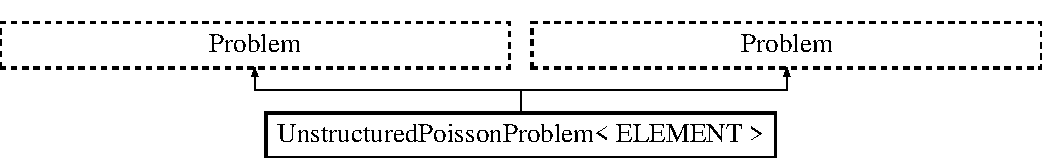
\includegraphics[height=2.000000cm]{classUnstructuredPoissonProblem}
\end{center}
\end{figure}
\subsection*{Public Member Functions}
\begin{DoxyCompactItemize}
\item 
\hyperlink{classUnstructuredPoissonProblem_a26e7610a714aea17c9278beec4842371}{Unstructured\+Poisson\+Problem} ()
\begin{DoxyCompactList}\small\item\em Constructor. \end{DoxyCompactList}\item 
\hyperlink{classUnstructuredPoissonProblem_aeae85592e36ba7be6b4891fb49d2197b}{$\sim$\+Unstructured\+Poisson\+Problem} ()
\begin{DoxyCompactList}\small\item\em Destructor. \end{DoxyCompactList}\item 
void \hyperlink{classUnstructuredPoissonProblem_ac9627efd3c311156e5347ed37d4ea4b0}{actions\+\_\+before\+\_\+adapt} ()
\begin{DoxyCompactList}\small\item\em Actions before adapt. Empty. \end{DoxyCompactList}\item 
void \hyperlink{classUnstructuredPoissonProblem_a6f3e089824cfbb4f458efd8c8ffd376d}{actions\+\_\+after\+\_\+adapt} ()
\begin{DoxyCompactList}\small\item\em Actions after adapt\+: Setup the problem again -- remember that the mesh has been completely rebuilt and its element\textquotesingle{}s don\textquotesingle{}t have any pointers to source fcts etc. yet. \end{DoxyCompactList}\item 
void \hyperlink{classUnstructuredPoissonProblem_a822bd18e50ebeefd6d1c196fad7c0bf1}{actions\+\_\+after\+\_\+newton\+\_\+solve} ()
\begin{DoxyCompactList}\small\item\em Update after solve (empty) \end{DoxyCompactList}\item 
void \hyperlink{classUnstructuredPoissonProblem_a2ab9d23c0e6e6631ffe1a761f6bdf026}{actions\+\_\+before\+\_\+newton\+\_\+solve} ()
\begin{DoxyCompactList}\small\item\em Update the problem specs before solve\+: Re-\/apply boundary conditons. \end{DoxyCompactList}\item 
void \hyperlink{classUnstructuredPoissonProblem_a9b21a3c3f574da71411f852006fe2a0c}{doc\+\_\+solution} (const std\+::string \&comment=\char`\"{}\char`\"{})
\begin{DoxyCompactList}\small\item\em Doc the solution. \end{DoxyCompactList}\item 
\hyperlink{classUnstructuredPoissonProblem_a26e7610a714aea17c9278beec4842371}{Unstructured\+Poisson\+Problem} ()
\begin{DoxyCompactList}\small\item\em Constructor. \end{DoxyCompactList}\item 
\hyperlink{classUnstructuredPoissonProblem_aeae85592e36ba7be6b4891fb49d2197b}{$\sim$\+Unstructured\+Poisson\+Problem} ()
\begin{DoxyCompactList}\small\item\em Destructor. \end{DoxyCompactList}\item 
void \hyperlink{classUnstructuredPoissonProblem_a822bd18e50ebeefd6d1c196fad7c0bf1}{actions\+\_\+after\+\_\+newton\+\_\+solve} ()
\begin{DoxyCompactList}\small\item\em Update after solve (empty) \end{DoxyCompactList}\item 
void \hyperlink{classUnstructuredPoissonProblem_a2ab9d23c0e6e6631ffe1a761f6bdf026}{actions\+\_\+before\+\_\+newton\+\_\+solve} ()
\begin{DoxyCompactList}\small\item\em Update the problem specs before solve\+: Re-\/apply boundary conditons. \end{DoxyCompactList}\item 
void \hyperlink{classUnstructuredPoissonProblem_a9b21a3c3f574da71411f852006fe2a0c}{doc\+\_\+solution} (const std\+::string \&comment=\char`\"{}\char`\"{})
\begin{DoxyCompactList}\small\item\em Doc the solution. \end{DoxyCompactList}\end{DoxyCompactItemize}
\subsection*{Private Member Functions}
\begin{DoxyCompactItemize}
\item 
void \hyperlink{classUnstructuredPoissonProblem_ace8b8b3097ae2024a0589b2bf9b4ee7b}{apply\+\_\+boundary\+\_\+conditions} ()
\begin{DoxyCompactList}\small\item\em Helper function to apply boundary conditions. \end{DoxyCompactList}\item 
void \hyperlink{classUnstructuredPoissonProblem_a5cbf00790e8469b43c64c6aaadfe7b41}{complete\+\_\+problem\+\_\+setup} ()
\begin{DoxyCompactList}\small\item\em Helper function to (re-\/)set boundary condition and complete the build of all elements. \end{DoxyCompactList}\item 
void \hyperlink{classUnstructuredPoissonProblem_ace8b8b3097ae2024a0589b2bf9b4ee7b}{apply\+\_\+boundary\+\_\+conditions} ()
\begin{DoxyCompactList}\small\item\em Helper function to apply boundary conditions. \end{DoxyCompactList}\item 
void \hyperlink{classUnstructuredPoissonProblem_a5cbf00790e8469b43c64c6aaadfe7b41}{complete\+\_\+problem\+\_\+setup} ()
\begin{DoxyCompactList}\small\item\em Helper function to (re-\/)set boundary condition and complete the build of all elements. \end{DoxyCompactList}\end{DoxyCompactItemize}
\subsection*{Private Attributes}
\begin{DoxyCompactItemize}
\item 
Doc\+Info \hyperlink{classUnstructuredPoissonProblem_a5c4c29b1c95cd63055e5aced124ca708}{Doc\+\_\+info}
\begin{DoxyCompactList}\small\item\em Doc info object for labeling output. \end{DoxyCompactList}\item 
Refineable\+Triangle\+Mesh$<$ E\+L\+E\+M\+E\+NT $>$ $\ast$ \hyperlink{classUnstructuredPoissonProblem_af95c713f5db16c288e307768b6bf9bb8}{My\+\_\+mesh\+\_\+pt}
\begin{DoxyCompactList}\small\item\em Pointers to specific mesh. \end{DoxyCompactList}\item 
ofstream \hyperlink{classUnstructuredPoissonProblem_ac7fdb8fb9a886ced0ee7244890406d90}{Trace\+\_\+file}
\begin{DoxyCompactList}\small\item\em Trace file to document norm of solution. \end{DoxyCompactList}\item 
Triangle\+Mesh$<$ E\+L\+E\+M\+E\+NT $>$ $\ast$ \hyperlink{classUnstructuredPoissonProblem_a138fcf0adb978a7f3ae9e27ba6df900b}{My\+\_\+mesh\+\_\+pt}
\begin{DoxyCompactList}\small\item\em Pointers to specific mesh. \end{DoxyCompactList}\end{DoxyCompactItemize}


\subsection{Detailed Description}
\subsubsection*{template$<$class E\+L\+E\+M\+E\+NT$>$\newline
class Unstructured\+Poisson\+Problem$<$ E\+L\+E\+M\+E\+N\+T $>$}

Class definition. 

Definition at line 94 of file mesh\+\_\+from\+\_\+inline\+\_\+triangle.\+cc.



\subsection{Constructor \& Destructor Documentation}
\mbox{\Hypertarget{classUnstructuredPoissonProblem_a26e7610a714aea17c9278beec4842371}\label{classUnstructuredPoissonProblem_a26e7610a714aea17c9278beec4842371}} 
\index{Unstructured\+Poisson\+Problem@{Unstructured\+Poisson\+Problem}!Unstructured\+Poisson\+Problem@{Unstructured\+Poisson\+Problem}}
\index{Unstructured\+Poisson\+Problem@{Unstructured\+Poisson\+Problem}!Unstructured\+Poisson\+Problem@{Unstructured\+Poisson\+Problem}}
\subsubsection{\texorpdfstring{Unstructured\+Poisson\+Problem()}{UnstructuredPoissonProblem()}\hspace{0.1cm}{\footnotesize\ttfamily [1/2]}}
{\footnotesize\ttfamily template$<$class E\+L\+E\+M\+E\+NT $>$ \\
\hyperlink{classUnstructuredPoissonProblem}{Unstructured\+Poisson\+Problem}$<$ E\+L\+E\+M\+E\+NT $>$\+::\hyperlink{classUnstructuredPoissonProblem}{Unstructured\+Poisson\+Problem} (\begin{DoxyParamCaption}{ }\end{DoxyParamCaption})}



Constructor. 



Definition at line 158 of file mesh\+\_\+from\+\_\+inline\+\_\+triangle.\+cc.

\mbox{\Hypertarget{classUnstructuredPoissonProblem_aeae85592e36ba7be6b4891fb49d2197b}\label{classUnstructuredPoissonProblem_aeae85592e36ba7be6b4891fb49d2197b}} 
\index{Unstructured\+Poisson\+Problem@{Unstructured\+Poisson\+Problem}!````~Unstructured\+Poisson\+Problem@{$\sim$\+Unstructured\+Poisson\+Problem}}
\index{````~Unstructured\+Poisson\+Problem@{$\sim$\+Unstructured\+Poisson\+Problem}!Unstructured\+Poisson\+Problem@{Unstructured\+Poisson\+Problem}}
\subsubsection{\texorpdfstring{$\sim$\+Unstructured\+Poisson\+Problem()}{~UnstructuredPoissonProblem()}\hspace{0.1cm}{\footnotesize\ttfamily [1/2]}}
{\footnotesize\ttfamily template$<$class E\+L\+E\+M\+E\+NT$>$ \\
\hyperlink{classUnstructuredPoissonProblem}{Unstructured\+Poisson\+Problem}$<$ E\+L\+E\+M\+E\+NT $>$\+::$\sim$\hyperlink{classUnstructuredPoissonProblem}{Unstructured\+Poisson\+Problem} (\begin{DoxyParamCaption}{ }\end{DoxyParamCaption})\hspace{0.3cm}{\ttfamily [inline]}}



Destructor. 



Definition at line 103 of file mesh\+\_\+from\+\_\+inline\+\_\+triangle.\+cc.

\mbox{\Hypertarget{classUnstructuredPoissonProblem_a26e7610a714aea17c9278beec4842371}\label{classUnstructuredPoissonProblem_a26e7610a714aea17c9278beec4842371}} 
\index{Unstructured\+Poisson\+Problem@{Unstructured\+Poisson\+Problem}!Unstructured\+Poisson\+Problem@{Unstructured\+Poisson\+Problem}}
\index{Unstructured\+Poisson\+Problem@{Unstructured\+Poisson\+Problem}!Unstructured\+Poisson\+Problem@{Unstructured\+Poisson\+Problem}}
\subsubsection{\texorpdfstring{Unstructured\+Poisson\+Problem()}{UnstructuredPoissonProblem()}\hspace{0.1cm}{\footnotesize\ttfamily [2/2]}}
{\footnotesize\ttfamily template$<$class E\+L\+E\+M\+E\+NT$>$ \\
\hyperlink{classUnstructuredPoissonProblem}{Unstructured\+Poisson\+Problem}$<$ E\+L\+E\+M\+E\+NT $>$\+::\hyperlink{classUnstructuredPoissonProblem}{Unstructured\+Poisson\+Problem} (\begin{DoxyParamCaption}{ }\end{DoxyParamCaption})}



Constructor. 

\mbox{\Hypertarget{classUnstructuredPoissonProblem_aeae85592e36ba7be6b4891fb49d2197b}\label{classUnstructuredPoissonProblem_aeae85592e36ba7be6b4891fb49d2197b}} 
\index{Unstructured\+Poisson\+Problem@{Unstructured\+Poisson\+Problem}!````~Unstructured\+Poisson\+Problem@{$\sim$\+Unstructured\+Poisson\+Problem}}
\index{````~Unstructured\+Poisson\+Problem@{$\sim$\+Unstructured\+Poisson\+Problem}!Unstructured\+Poisson\+Problem@{Unstructured\+Poisson\+Problem}}
\subsubsection{\texorpdfstring{$\sim$\+Unstructured\+Poisson\+Problem()}{~UnstructuredPoissonProblem()}\hspace{0.1cm}{\footnotesize\ttfamily [2/2]}}
{\footnotesize\ttfamily template$<$class E\+L\+E\+M\+E\+NT$>$ \\
\hyperlink{classUnstructuredPoissonProblem}{Unstructured\+Poisson\+Problem}$<$ E\+L\+E\+M\+E\+NT $>$\+::$\sim$\hyperlink{classUnstructuredPoissonProblem}{Unstructured\+Poisson\+Problem} (\begin{DoxyParamCaption}{ }\end{DoxyParamCaption})\hspace{0.3cm}{\ttfamily [inline]}}



Destructor. 



Definition at line 103 of file mesh\+\_\+from\+\_\+inline\+\_\+triangle\+\_\+no\+\_\+adapt.\+cc.



\subsection{Member Function Documentation}
\mbox{\Hypertarget{classUnstructuredPoissonProblem_a6f3e089824cfbb4f458efd8c8ffd376d}\label{classUnstructuredPoissonProblem_a6f3e089824cfbb4f458efd8c8ffd376d}} 
\index{Unstructured\+Poisson\+Problem@{Unstructured\+Poisson\+Problem}!actions\+\_\+after\+\_\+adapt@{actions\+\_\+after\+\_\+adapt}}
\index{actions\+\_\+after\+\_\+adapt@{actions\+\_\+after\+\_\+adapt}!Unstructured\+Poisson\+Problem@{Unstructured\+Poisson\+Problem}}
\subsubsection{\texorpdfstring{actions\+\_\+after\+\_\+adapt()}{actions\_after\_adapt()}}
{\footnotesize\ttfamily template$<$class E\+L\+E\+M\+E\+NT$>$ \\
void \hyperlink{classUnstructuredPoissonProblem}{Unstructured\+Poisson\+Problem}$<$ E\+L\+E\+M\+E\+NT $>$\+::actions\+\_\+after\+\_\+adapt (\begin{DoxyParamCaption}{ }\end{DoxyParamCaption})\hspace{0.3cm}{\ttfamily [inline]}}



Actions after adapt\+: Setup the problem again -- remember that the mesh has been completely rebuilt and its element\textquotesingle{}s don\textquotesingle{}t have any pointers to source fcts etc. yet. 



Definition at line 112 of file mesh\+\_\+from\+\_\+inline\+\_\+triangle.\+cc.

\mbox{\Hypertarget{classUnstructuredPoissonProblem_a822bd18e50ebeefd6d1c196fad7c0bf1}\label{classUnstructuredPoissonProblem_a822bd18e50ebeefd6d1c196fad7c0bf1}} 
\index{Unstructured\+Poisson\+Problem@{Unstructured\+Poisson\+Problem}!actions\+\_\+after\+\_\+newton\+\_\+solve@{actions\+\_\+after\+\_\+newton\+\_\+solve}}
\index{actions\+\_\+after\+\_\+newton\+\_\+solve@{actions\+\_\+after\+\_\+newton\+\_\+solve}!Unstructured\+Poisson\+Problem@{Unstructured\+Poisson\+Problem}}
\subsubsection{\texorpdfstring{actions\+\_\+after\+\_\+newton\+\_\+solve()}{actions\_after\_newton\_solve()}\hspace{0.1cm}{\footnotesize\ttfamily [1/2]}}
{\footnotesize\ttfamily template$<$class E\+L\+E\+M\+E\+NT$>$ \\
void \hyperlink{classUnstructuredPoissonProblem}{Unstructured\+Poisson\+Problem}$<$ E\+L\+E\+M\+E\+NT $>$\+::actions\+\_\+after\+\_\+newton\+\_\+solve (\begin{DoxyParamCaption}{ }\end{DoxyParamCaption})\hspace{0.3cm}{\ttfamily [inline]}}



Update after solve (empty) 



Definition at line 106 of file mesh\+\_\+from\+\_\+inline\+\_\+triangle\+\_\+no\+\_\+adapt.\+cc.

\mbox{\Hypertarget{classUnstructuredPoissonProblem_a822bd18e50ebeefd6d1c196fad7c0bf1}\label{classUnstructuredPoissonProblem_a822bd18e50ebeefd6d1c196fad7c0bf1}} 
\index{Unstructured\+Poisson\+Problem@{Unstructured\+Poisson\+Problem}!actions\+\_\+after\+\_\+newton\+\_\+solve@{actions\+\_\+after\+\_\+newton\+\_\+solve}}
\index{actions\+\_\+after\+\_\+newton\+\_\+solve@{actions\+\_\+after\+\_\+newton\+\_\+solve}!Unstructured\+Poisson\+Problem@{Unstructured\+Poisson\+Problem}}
\subsubsection{\texorpdfstring{actions\+\_\+after\+\_\+newton\+\_\+solve()}{actions\_after\_newton\_solve()}\hspace{0.1cm}{\footnotesize\ttfamily [2/2]}}
{\footnotesize\ttfamily template$<$class E\+L\+E\+M\+E\+NT$>$ \\
void \hyperlink{classUnstructuredPoissonProblem}{Unstructured\+Poisson\+Problem}$<$ E\+L\+E\+M\+E\+NT $>$\+::actions\+\_\+after\+\_\+newton\+\_\+solve (\begin{DoxyParamCaption}{ }\end{DoxyParamCaption})\hspace{0.3cm}{\ttfamily [inline]}}



Update after solve (empty) 



Definition at line 118 of file mesh\+\_\+from\+\_\+inline\+\_\+triangle.\+cc.

\mbox{\Hypertarget{classUnstructuredPoissonProblem_ac9627efd3c311156e5347ed37d4ea4b0}\label{classUnstructuredPoissonProblem_ac9627efd3c311156e5347ed37d4ea4b0}} 
\index{Unstructured\+Poisson\+Problem@{Unstructured\+Poisson\+Problem}!actions\+\_\+before\+\_\+adapt@{actions\+\_\+before\+\_\+adapt}}
\index{actions\+\_\+before\+\_\+adapt@{actions\+\_\+before\+\_\+adapt}!Unstructured\+Poisson\+Problem@{Unstructured\+Poisson\+Problem}}
\subsubsection{\texorpdfstring{actions\+\_\+before\+\_\+adapt()}{actions\_before\_adapt()}}
{\footnotesize\ttfamily template$<$class E\+L\+E\+M\+E\+NT$>$ \\
void \hyperlink{classUnstructuredPoissonProblem}{Unstructured\+Poisson\+Problem}$<$ E\+L\+E\+M\+E\+NT $>$\+::actions\+\_\+before\+\_\+adapt (\begin{DoxyParamCaption}{ }\end{DoxyParamCaption})\hspace{0.3cm}{\ttfamily [inline]}}



Actions before adapt. Empty. 



Definition at line 106 of file mesh\+\_\+from\+\_\+inline\+\_\+triangle.\+cc.

\mbox{\Hypertarget{classUnstructuredPoissonProblem_a2ab9d23c0e6e6631ffe1a761f6bdf026}\label{classUnstructuredPoissonProblem_a2ab9d23c0e6e6631ffe1a761f6bdf026}} 
\index{Unstructured\+Poisson\+Problem@{Unstructured\+Poisson\+Problem}!actions\+\_\+before\+\_\+newton\+\_\+solve@{actions\+\_\+before\+\_\+newton\+\_\+solve}}
\index{actions\+\_\+before\+\_\+newton\+\_\+solve@{actions\+\_\+before\+\_\+newton\+\_\+solve}!Unstructured\+Poisson\+Problem@{Unstructured\+Poisson\+Problem}}
\subsubsection{\texorpdfstring{actions\+\_\+before\+\_\+newton\+\_\+solve()}{actions\_before\_newton\_solve()}\hspace{0.1cm}{\footnotesize\ttfamily [1/2]}}
{\footnotesize\ttfamily template$<$class E\+L\+E\+M\+E\+NT$>$ \\
void \hyperlink{classUnstructuredPoissonProblem}{Unstructured\+Poisson\+Problem}$<$ E\+L\+E\+M\+E\+NT $>$\+::actions\+\_\+before\+\_\+newton\+\_\+solve (\begin{DoxyParamCaption}{ }\end{DoxyParamCaption})\hspace{0.3cm}{\ttfamily [inline]}}



Update the problem specs before solve\+: Re-\/apply boundary conditons. 



Definition at line 109 of file mesh\+\_\+from\+\_\+inline\+\_\+triangle\+\_\+no\+\_\+adapt.\+cc.

\mbox{\Hypertarget{classUnstructuredPoissonProblem_a2ab9d23c0e6e6631ffe1a761f6bdf026}\label{classUnstructuredPoissonProblem_a2ab9d23c0e6e6631ffe1a761f6bdf026}} 
\index{Unstructured\+Poisson\+Problem@{Unstructured\+Poisson\+Problem}!actions\+\_\+before\+\_\+newton\+\_\+solve@{actions\+\_\+before\+\_\+newton\+\_\+solve}}
\index{actions\+\_\+before\+\_\+newton\+\_\+solve@{actions\+\_\+before\+\_\+newton\+\_\+solve}!Unstructured\+Poisson\+Problem@{Unstructured\+Poisson\+Problem}}
\subsubsection{\texorpdfstring{actions\+\_\+before\+\_\+newton\+\_\+solve()}{actions\_before\_newton\_solve()}\hspace{0.1cm}{\footnotesize\ttfamily [2/2]}}
{\footnotesize\ttfamily template$<$class E\+L\+E\+M\+E\+NT$>$ \\
void \hyperlink{classUnstructuredPoissonProblem}{Unstructured\+Poisson\+Problem}$<$ E\+L\+E\+M\+E\+NT $>$\+::actions\+\_\+before\+\_\+newton\+\_\+solve (\begin{DoxyParamCaption}{ }\end{DoxyParamCaption})\hspace{0.3cm}{\ttfamily [inline]}}



Update the problem specs before solve\+: Re-\/apply boundary conditons. 



Definition at line 121 of file mesh\+\_\+from\+\_\+inline\+\_\+triangle.\+cc.

\mbox{\Hypertarget{classUnstructuredPoissonProblem_ace8b8b3097ae2024a0589b2bf9b4ee7b}\label{classUnstructuredPoissonProblem_ace8b8b3097ae2024a0589b2bf9b4ee7b}} 
\index{Unstructured\+Poisson\+Problem@{Unstructured\+Poisson\+Problem}!apply\+\_\+boundary\+\_\+conditions@{apply\+\_\+boundary\+\_\+conditions}}
\index{apply\+\_\+boundary\+\_\+conditions@{apply\+\_\+boundary\+\_\+conditions}!Unstructured\+Poisson\+Problem@{Unstructured\+Poisson\+Problem}}
\subsubsection{\texorpdfstring{apply\+\_\+boundary\+\_\+conditions()}{apply\_boundary\_conditions()}\hspace{0.1cm}{\footnotesize\ttfamily [1/2]}}
{\footnotesize\ttfamily template$<$class E\+L\+E\+M\+E\+NT$>$ \\
void \hyperlink{classUnstructuredPoissonProblem}{Unstructured\+Poisson\+Problem}$<$ E\+L\+E\+M\+E\+NT $>$\+::apply\+\_\+boundary\+\_\+conditions (\begin{DoxyParamCaption}{ }\end{DoxyParamCaption})\hspace{0.3cm}{\ttfamily [private]}}



Helper function to apply boundary conditions. 

\mbox{\Hypertarget{classUnstructuredPoissonProblem_ace8b8b3097ae2024a0589b2bf9b4ee7b}\label{classUnstructuredPoissonProblem_ace8b8b3097ae2024a0589b2bf9b4ee7b}} 
\index{Unstructured\+Poisson\+Problem@{Unstructured\+Poisson\+Problem}!apply\+\_\+boundary\+\_\+conditions@{apply\+\_\+boundary\+\_\+conditions}}
\index{apply\+\_\+boundary\+\_\+conditions@{apply\+\_\+boundary\+\_\+conditions}!Unstructured\+Poisson\+Problem@{Unstructured\+Poisson\+Problem}}
\subsubsection{\texorpdfstring{apply\+\_\+boundary\+\_\+conditions()}{apply\_boundary\_conditions()}\hspace{0.1cm}{\footnotesize\ttfamily [2/2]}}
{\footnotesize\ttfamily template$<$class E\+L\+E\+M\+E\+NT $>$ \\
void \hyperlink{classUnstructuredPoissonProblem}{Unstructured\+Poisson\+Problem}$<$ E\+L\+E\+M\+E\+NT $>$\+::apply\+\_\+boundary\+\_\+conditions (\begin{DoxyParamCaption}{ }\end{DoxyParamCaption})\hspace{0.3cm}{\ttfamily [private]}}



Helper function to apply boundary conditions. 



Definition at line 506 of file mesh\+\_\+from\+\_\+inline\+\_\+triangle.\+cc.



References Tanh\+Soln\+For\+Poisson\+::get\+\_\+exact\+\_\+u().

\mbox{\Hypertarget{classUnstructuredPoissonProblem_a5cbf00790e8469b43c64c6aaadfe7b41}\label{classUnstructuredPoissonProblem_a5cbf00790e8469b43c64c6aaadfe7b41}} 
\index{Unstructured\+Poisson\+Problem@{Unstructured\+Poisson\+Problem}!complete\+\_\+problem\+\_\+setup@{complete\+\_\+problem\+\_\+setup}}
\index{complete\+\_\+problem\+\_\+setup@{complete\+\_\+problem\+\_\+setup}!Unstructured\+Poisson\+Problem@{Unstructured\+Poisson\+Problem}}
\subsubsection{\texorpdfstring{complete\+\_\+problem\+\_\+setup()}{complete\_problem\_setup()}\hspace{0.1cm}{\footnotesize\ttfamily [1/2]}}
{\footnotesize\ttfamily template$<$class E\+L\+E\+M\+E\+NT$>$ \\
void \hyperlink{classUnstructuredPoissonProblem}{Unstructured\+Poisson\+Problem}$<$ E\+L\+E\+M\+E\+NT $>$\+::complete\+\_\+problem\+\_\+setup (\begin{DoxyParamCaption}{ }\end{DoxyParamCaption})\hspace{0.3cm}{\ttfamily [private]}}



Helper function to (re-\/)set boundary condition and complete the build of all elements. 

\mbox{\Hypertarget{classUnstructuredPoissonProblem_a5cbf00790e8469b43c64c6aaadfe7b41}\label{classUnstructuredPoissonProblem_a5cbf00790e8469b43c64c6aaadfe7b41}} 
\index{Unstructured\+Poisson\+Problem@{Unstructured\+Poisson\+Problem}!complete\+\_\+problem\+\_\+setup@{complete\+\_\+problem\+\_\+setup}}
\index{complete\+\_\+problem\+\_\+setup@{complete\+\_\+problem\+\_\+setup}!Unstructured\+Poisson\+Problem@{Unstructured\+Poisson\+Problem}}
\subsubsection{\texorpdfstring{complete\+\_\+problem\+\_\+setup()}{complete\_problem\_setup()}\hspace{0.1cm}{\footnotesize\ttfamily [2/2]}}
{\footnotesize\ttfamily template$<$class E\+L\+E\+M\+E\+NT $>$ \\
void \hyperlink{classUnstructuredPoissonProblem}{Unstructured\+Poisson\+Problem}$<$ E\+L\+E\+M\+E\+NT $>$\+::complete\+\_\+problem\+\_\+setup (\begin{DoxyParamCaption}{ }\end{DoxyParamCaption})\hspace{0.3cm}{\ttfamily [private]}}



Helper function to (re-\/)set boundary condition and complete the build of all elements. 

Set boundary condition exactly, and complete the build of all elements 

Definition at line 462 of file mesh\+\_\+from\+\_\+inline\+\_\+triangle.\+cc.



References Tanh\+Soln\+For\+Poisson\+::get\+\_\+source().

\mbox{\Hypertarget{classUnstructuredPoissonProblem_a9b21a3c3f574da71411f852006fe2a0c}\label{classUnstructuredPoissonProblem_a9b21a3c3f574da71411f852006fe2a0c}} 
\index{Unstructured\+Poisson\+Problem@{Unstructured\+Poisson\+Problem}!doc\+\_\+solution@{doc\+\_\+solution}}
\index{doc\+\_\+solution@{doc\+\_\+solution}!Unstructured\+Poisson\+Problem@{Unstructured\+Poisson\+Problem}}
\subsubsection{\texorpdfstring{doc\+\_\+solution()}{doc\_solution()}\hspace{0.1cm}{\footnotesize\ttfamily [1/2]}}
{\footnotesize\ttfamily template$<$class E\+L\+E\+M\+E\+NT$>$ \\
void \hyperlink{classUnstructuredPoissonProblem}{Unstructured\+Poisson\+Problem}$<$ E\+L\+E\+M\+E\+NT $>$\+::doc\+\_\+solution (\begin{DoxyParamCaption}\item[{const std\+::string \&}]{comment = {\ttfamily \char`\"{}\char`\"{}} }\end{DoxyParamCaption})}



Doc the solution. 

\mbox{\Hypertarget{classUnstructuredPoissonProblem_a9b21a3c3f574da71411f852006fe2a0c}\label{classUnstructuredPoissonProblem_a9b21a3c3f574da71411f852006fe2a0c}} 
\index{Unstructured\+Poisson\+Problem@{Unstructured\+Poisson\+Problem}!doc\+\_\+solution@{doc\+\_\+solution}}
\index{doc\+\_\+solution@{doc\+\_\+solution}!Unstructured\+Poisson\+Problem@{Unstructured\+Poisson\+Problem}}
\subsubsection{\texorpdfstring{doc\+\_\+solution()}{doc\_solution()}\hspace{0.1cm}{\footnotesize\ttfamily [2/2]}}
{\footnotesize\ttfamily template$<$class E\+L\+E\+M\+E\+NT $>$ \\
void \hyperlink{classUnstructuredPoissonProblem}{Unstructured\+Poisson\+Problem}$<$ E\+L\+E\+M\+E\+NT $>$\+::doc\+\_\+solution (\begin{DoxyParamCaption}\item[{const std\+::string \&}]{comment = {\ttfamily \char`\"{}\char`\"{}} }\end{DoxyParamCaption})}



Doc the solution. 



Definition at line 540 of file mesh\+\_\+from\+\_\+inline\+\_\+triangle.\+cc.



References Tanh\+Soln\+For\+Poisson\+::get\+\_\+exact\+\_\+u(), and Tanh\+Soln\+For\+Poisson\+::zero().



Referenced by main().



\subsection{Member Data Documentation}
\mbox{\Hypertarget{classUnstructuredPoissonProblem_a5c4c29b1c95cd63055e5aced124ca708}\label{classUnstructuredPoissonProblem_a5c4c29b1c95cd63055e5aced124ca708}} 
\index{Unstructured\+Poisson\+Problem@{Unstructured\+Poisson\+Problem}!Doc\+\_\+info@{Doc\+\_\+info}}
\index{Doc\+\_\+info@{Doc\+\_\+info}!Unstructured\+Poisson\+Problem@{Unstructured\+Poisson\+Problem}}
\subsubsection{\texorpdfstring{Doc\+\_\+info}{Doc\_info}}
{\footnotesize\ttfamily template$<$class E\+L\+E\+M\+E\+NT$>$ \\
Doc\+Info \hyperlink{classUnstructuredPoissonProblem}{Unstructured\+Poisson\+Problem}$<$ E\+L\+E\+M\+E\+NT $>$\+::Doc\+\_\+info\hspace{0.3cm}{\ttfamily [private]}}



Doc info object for labeling output. 



Definition at line 133 of file mesh\+\_\+from\+\_\+inline\+\_\+triangle.\+cc.

\mbox{\Hypertarget{classUnstructuredPoissonProblem_a138fcf0adb978a7f3ae9e27ba6df900b}\label{classUnstructuredPoissonProblem_a138fcf0adb978a7f3ae9e27ba6df900b}} 
\index{Unstructured\+Poisson\+Problem@{Unstructured\+Poisson\+Problem}!My\+\_\+mesh\+\_\+pt@{My\+\_\+mesh\+\_\+pt}}
\index{My\+\_\+mesh\+\_\+pt@{My\+\_\+mesh\+\_\+pt}!Unstructured\+Poisson\+Problem@{Unstructured\+Poisson\+Problem}}
\subsubsection{\texorpdfstring{My\+\_\+mesh\+\_\+pt}{My\_mesh\_pt}\hspace{0.1cm}{\footnotesize\ttfamily [1/2]}}
{\footnotesize\ttfamily template$<$class E\+L\+E\+M\+E\+NT$>$ \\
Triangle\+Mesh$<$E\+L\+E\+M\+E\+NT$>$$\ast$ \hyperlink{classUnstructuredPoissonProblem}{Unstructured\+Poisson\+Problem}$<$ E\+L\+E\+M\+E\+NT $>$\+::My\+\_\+mesh\+\_\+pt\hspace{0.3cm}{\ttfamily [private]}}



Pointers to specific mesh. 



Definition at line 131 of file mesh\+\_\+from\+\_\+inline\+\_\+triangle\+\_\+no\+\_\+adapt.\+cc.

\mbox{\Hypertarget{classUnstructuredPoissonProblem_af95c713f5db16c288e307768b6bf9bb8}\label{classUnstructuredPoissonProblem_af95c713f5db16c288e307768b6bf9bb8}} 
\index{Unstructured\+Poisson\+Problem@{Unstructured\+Poisson\+Problem}!My\+\_\+mesh\+\_\+pt@{My\+\_\+mesh\+\_\+pt}}
\index{My\+\_\+mesh\+\_\+pt@{My\+\_\+mesh\+\_\+pt}!Unstructured\+Poisson\+Problem@{Unstructured\+Poisson\+Problem}}
\subsubsection{\texorpdfstring{My\+\_\+mesh\+\_\+pt}{My\_mesh\_pt}\hspace{0.1cm}{\footnotesize\ttfamily [2/2]}}
{\footnotesize\ttfamily template$<$class E\+L\+E\+M\+E\+NT$>$ \\
Refineable\+Triangle\+Mesh$<$E\+L\+E\+M\+E\+NT$>$$\ast$ \hyperlink{classUnstructuredPoissonProblem}{Unstructured\+Poisson\+Problem}$<$ E\+L\+E\+M\+E\+NT $>$\+::My\+\_\+mesh\+\_\+pt\hspace{0.3cm}{\ttfamily [private]}}



Pointers to specific mesh. 



Definition at line 143 of file mesh\+\_\+from\+\_\+inline\+\_\+triangle.\+cc.

\mbox{\Hypertarget{classUnstructuredPoissonProblem_ac7fdb8fb9a886ced0ee7244890406d90}\label{classUnstructuredPoissonProblem_ac7fdb8fb9a886ced0ee7244890406d90}} 
\index{Unstructured\+Poisson\+Problem@{Unstructured\+Poisson\+Problem}!Trace\+\_\+file@{Trace\+\_\+file}}
\index{Trace\+\_\+file@{Trace\+\_\+file}!Unstructured\+Poisson\+Problem@{Unstructured\+Poisson\+Problem}}
\subsubsection{\texorpdfstring{Trace\+\_\+file}{Trace\_file}}
{\footnotesize\ttfamily template$<$class E\+L\+E\+M\+E\+NT$>$ \\
ofstream \hyperlink{classUnstructuredPoissonProblem}{Unstructured\+Poisson\+Problem}$<$ E\+L\+E\+M\+E\+NT $>$\+::Trace\+\_\+file\hspace{0.3cm}{\ttfamily [private]}}



Trace file to document norm of solution. 



Definition at line 146 of file mesh\+\_\+from\+\_\+inline\+\_\+triangle.\+cc.



The documentation for this class was generated from the following files\+:\begin{DoxyCompactItemize}
\item 
\hyperlink{mesh__from__inline__triangle_8cc}{mesh\+\_\+from\+\_\+inline\+\_\+triangle.\+cc}\item 
\hyperlink{mesh__from__inline__triangle__no__adapt_8cc}{mesh\+\_\+from\+\_\+inline\+\_\+triangle\+\_\+no\+\_\+adapt.\+cc}\end{DoxyCompactItemize}

\chapter{File Documentation}
\hypertarget{mesh__from__inline__triangle_8cc}{}\section{mesh\+\_\+from\+\_\+inline\+\_\+triangle.\+cc File Reference}
\label{mesh__from__inline__triangle_8cc}\index{mesh\+\_\+from\+\_\+inline\+\_\+triangle.\+cc@{mesh\+\_\+from\+\_\+inline\+\_\+triangle.\+cc}}
\subsection*{Classes}
\begin{DoxyCompactItemize}
\item 
class \hyperlink{classUnstructuredPoissonProblem}{Unstructured\+Poisson\+Problem$<$ E\+L\+E\+M\+E\+N\+T $>$}
\begin{DoxyCompactList}\small\item\em Class definition. \end{DoxyCompactList}\end{DoxyCompactItemize}
\subsection*{Namespaces}
\begin{DoxyCompactItemize}
\item 
 \hyperlink{namespaceTanhSolnForPoisson}{Tanh\+Soln\+For\+Poisson}
\begin{DoxyCompactList}\small\item\em Namespace for exact solution for Poisson equation with \char`\"{}sharp step\char`\"{}. \end{DoxyCompactList}\end{DoxyCompactItemize}
\subsection*{Functions}
\begin{DoxyCompactItemize}
\item 
void \hyperlink{namespaceTanhSolnForPoisson_af7896e9c18ce6438c73ae2a875e8b7de}{Tanh\+Soln\+For\+Poisson\+::get\+\_\+exact\+\_\+u} (const Vector$<$ double $>$ \&x, Vector$<$ double $>$ \&u)
\begin{DoxyCompactList}\small\item\em Exact solution as a Vector. \end{DoxyCompactList}\item 
void \hyperlink{namespaceTanhSolnForPoisson_ae1b9d6789ff301e3d63a4e292213036c}{Tanh\+Soln\+For\+Poisson\+::get\+\_\+source} (const Vector$<$ double $>$ \&x, double \&source)
\begin{DoxyCompactList}\small\item\em Source function required to make the solution above an exact solution. \end{DoxyCompactList}\item 
void \hyperlink{namespaceTanhSolnForPoisson_a5cd8441c6e87d4bc153697eff13513dd}{Tanh\+Soln\+For\+Poisson\+::zero} (const Vector$<$ double $>$ \&x, Vector$<$ double $>$ \&u)
\begin{DoxyCompactList}\small\item\em Zero function -- used to compute norm of the computed solution by computing the norm of the error when compared against this. \end{DoxyCompactList}\item 
int \hyperlink{mesh__from__inline__triangle_8cc_a3c04138a5bfe5d72780bb7e82a18e627}{main} (int argc, char $\ast$$\ast$argv)
\begin{DoxyCompactList}\small\item\em Driver code for demo of inline triangle mesh generation. \end{DoxyCompactList}\end{DoxyCompactItemize}
\subsection*{Variables}
\begin{DoxyCompactItemize}
\item 
double \hyperlink{namespaceTanhSolnForPoisson_ae676ccd186d5df119cce811596d949c1}{Tanh\+Soln\+For\+Poisson\+::\+Alpha} =5.\+0
\begin{DoxyCompactList}\small\item\em Parameter for steepness of \char`\"{}step\char`\"{}. \end{DoxyCompactList}\item 
double \hyperlink{namespaceTanhSolnForPoisson_a785ccd00a727125a5138fbbcac173294}{Tanh\+Soln\+For\+Poisson\+::\+Tan\+Phi} =0.\+0
\begin{DoxyCompactList}\small\item\em Parameter for angle Phi of \char`\"{}step\char`\"{}. \end{DoxyCompactList}\end{DoxyCompactItemize}


\subsection{Function Documentation}
\mbox{\Hypertarget{mesh__from__inline__triangle_8cc_a3c04138a5bfe5d72780bb7e82a18e627}\label{mesh__from__inline__triangle_8cc_a3c04138a5bfe5d72780bb7e82a18e627}} 
\index{mesh\+\_\+from\+\_\+inline\+\_\+triangle.\+cc@{mesh\+\_\+from\+\_\+inline\+\_\+triangle.\+cc}!main@{main}}
\index{main@{main}!mesh\+\_\+from\+\_\+inline\+\_\+triangle.\+cc@{mesh\+\_\+from\+\_\+inline\+\_\+triangle.\+cc}}
\subsubsection{\texorpdfstring{main()}{main()}}
{\footnotesize\ttfamily int main (\begin{DoxyParamCaption}\item[{int}]{argc,  }\item[{char $\ast$$\ast$}]{argv }\end{DoxyParamCaption})}



Driver code for demo of inline triangle mesh generation. 



Definition at line 599 of file mesh\+\_\+from\+\_\+inline\+\_\+triangle.\+cc.



References Unstructured\+Poisson\+Problem$<$ E\+L\+E\+M\+E\+N\+T $>$\+::doc\+\_\+solution(), and Tanh\+Soln\+For\+Poisson\+::\+Tan\+Phi.


\hypertarget{mesh__from__inline__triangle_8txt__doxygenified_8h}{}\section{mesh\+\_\+from\+\_\+inline\+\_\+triangle.\+txt\+\_\+doxygenified.\+h File Reference}
\label{mesh__from__inline__triangle_8txt__doxygenified_8h}\index{mesh\+\_\+from\+\_\+inline\+\_\+triangle.\+txt\+\_\+doxygenified.\+h@{mesh\+\_\+from\+\_\+inline\+\_\+triangle.\+txt\+\_\+doxygenified.\+h}}

\hypertarget{mesh__from__inline__triangle__no__adapt_8cc}{}\section{mesh\+\_\+from\+\_\+inline\+\_\+triangle\+\_\+no\+\_\+adapt.\+cc File Reference}
\label{mesh__from__inline__triangle__no__adapt_8cc}\index{mesh\+\_\+from\+\_\+inline\+\_\+triangle\+\_\+no\+\_\+adapt.\+cc@{mesh\+\_\+from\+\_\+inline\+\_\+triangle\+\_\+no\+\_\+adapt.\+cc}}
\subsection*{Classes}
\begin{DoxyCompactItemize}
\item 
class \hyperlink{classUnstructuredPoissonProblem}{Unstructured\+Poisson\+Problem$<$ E\+L\+E\+M\+E\+N\+T $>$}
\begin{DoxyCompactList}\small\item\em Class definition. \end{DoxyCompactList}\end{DoxyCompactItemize}
\subsection*{Namespaces}
\begin{DoxyCompactItemize}
\item 
 \hyperlink{namespaceTanhSolnForPoisson}{Tanh\+Soln\+For\+Poisson}
\begin{DoxyCompactList}\small\item\em Namespace for exact solution for Poisson equation with \char`\"{}sharp step\char`\"{}. \end{DoxyCompactList}\end{DoxyCompactItemize}
\subsection*{Functions}
\begin{DoxyCompactItemize}
\item 
void \hyperlink{namespaceTanhSolnForPoisson_af7896e9c18ce6438c73ae2a875e8b7de}{Tanh\+Soln\+For\+Poisson\+::get\+\_\+exact\+\_\+u} (const Vector$<$ double $>$ \&x, Vector$<$ double $>$ \&u)
\begin{DoxyCompactList}\small\item\em Exact solution as a Vector. \end{DoxyCompactList}\item 
void \hyperlink{namespaceTanhSolnForPoisson_ae1b9d6789ff301e3d63a4e292213036c}{Tanh\+Soln\+For\+Poisson\+::get\+\_\+source} (const Vector$<$ double $>$ \&x, double \&source)
\begin{DoxyCompactList}\small\item\em Source function required to make the solution above an exact solution. \end{DoxyCompactList}\item 
void \hyperlink{namespaceTanhSolnForPoisson_a5cd8441c6e87d4bc153697eff13513dd}{Tanh\+Soln\+For\+Poisson\+::zero} (const Vector$<$ double $>$ \&x, Vector$<$ double $>$ \&u)
\begin{DoxyCompactList}\small\item\em Zero function -- used to compute norm of the computed solution by computing the norm of the error when compared against this. \end{DoxyCompactList}\item 
int \hyperlink{mesh__from__inline__triangle__no__adapt_8cc_a3c04138a5bfe5d72780bb7e82a18e627}{main} (int argc, char $\ast$$\ast$argv)
\begin{DoxyCompactList}\small\item\em Driver code for demo of inline triangle mesh generation. \end{DoxyCompactList}\end{DoxyCompactItemize}


\subsection{Function Documentation}
\mbox{\Hypertarget{mesh__from__inline__triangle__no__adapt_8cc_a3c04138a5bfe5d72780bb7e82a18e627}\label{mesh__from__inline__triangle__no__adapt_8cc_a3c04138a5bfe5d72780bb7e82a18e627}} 
\index{mesh\+\_\+from\+\_\+inline\+\_\+triangle\+\_\+no\+\_\+adapt.\+cc@{mesh\+\_\+from\+\_\+inline\+\_\+triangle\+\_\+no\+\_\+adapt.\+cc}!main@{main}}
\index{main@{main}!mesh\+\_\+from\+\_\+inline\+\_\+triangle\+\_\+no\+\_\+adapt.\+cc@{mesh\+\_\+from\+\_\+inline\+\_\+triangle\+\_\+no\+\_\+adapt.\+cc}}
\subsubsection{\texorpdfstring{main()}{main()}}
{\footnotesize\ttfamily int main (\begin{DoxyParamCaption}\item[{int}]{argc,  }\item[{char $\ast$$\ast$}]{argv }\end{DoxyParamCaption})}



Driver code for demo of inline triangle mesh generation. 



Definition at line 577 of file mesh\+\_\+from\+\_\+inline\+\_\+triangle\+\_\+no\+\_\+adapt.\+cc.



References Unstructured\+Poisson\+Problem$<$ E\+L\+E\+M\+E\+N\+T $>$\+::doc\+\_\+solution(), and Tanh\+Soln\+For\+Poisson\+::\+Tan\+Phi.


\hypertarget{projection_8h}{}\section{projection.\+h File Reference}
\label{projection_8h}\index{projection.\+h@{projection.\+h}}
\subsection*{Classes}
\begin{DoxyCompactItemize}
\item 
class \hyperlink{classoomph_1_1ProjectableElementBase}{oomph\+::\+Projectable\+Element\+Base}
\begin{DoxyCompactList}\small\item\em Template-\/free Base class for projectable elements. \end{DoxyCompactList}\item 
class \hyperlink{classoomph_1_1ProjectableElement}{oomph\+::\+Projectable\+Element$<$ E\+L\+E\+M\+E\+N\+T $>$}
\item 
class \hyperlink{classoomph_1_1FaceGeometry_3_01ProjectableElement_3_01ELEMENT_01_4_01_4}{oomph\+::\+Face\+Geometry$<$ Projectable\+Element$<$ E\+L\+E\+M\+E\+N\+T $>$ $>$}
\item 
class \hyperlink{classoomph_1_1ProjectionProblem}{oomph\+::\+Projection\+Problem$<$ P\+R\+O\+J\+E\+C\+T\+A\+B\+L\+E\+\_\+\+E\+L\+E\+M\+E\+N\+T $>$}
\end{DoxyCompactItemize}
\subsection*{Namespaces}
\begin{DoxyCompactItemize}
\item 
 \hyperlink{namespaceoomph}{oomph}
\end{DoxyCompactItemize}

%--- End generated contents ---

% Index
\backmatter
\newpage
\phantomsection
\clearemptydoublepage
\addcontentsline{toc}{chapter}{Index}
\printindex

\end{document}
